\section{Piede piatto}

\subsection{Definizione}

\begin{figure}[!ht]
\centering
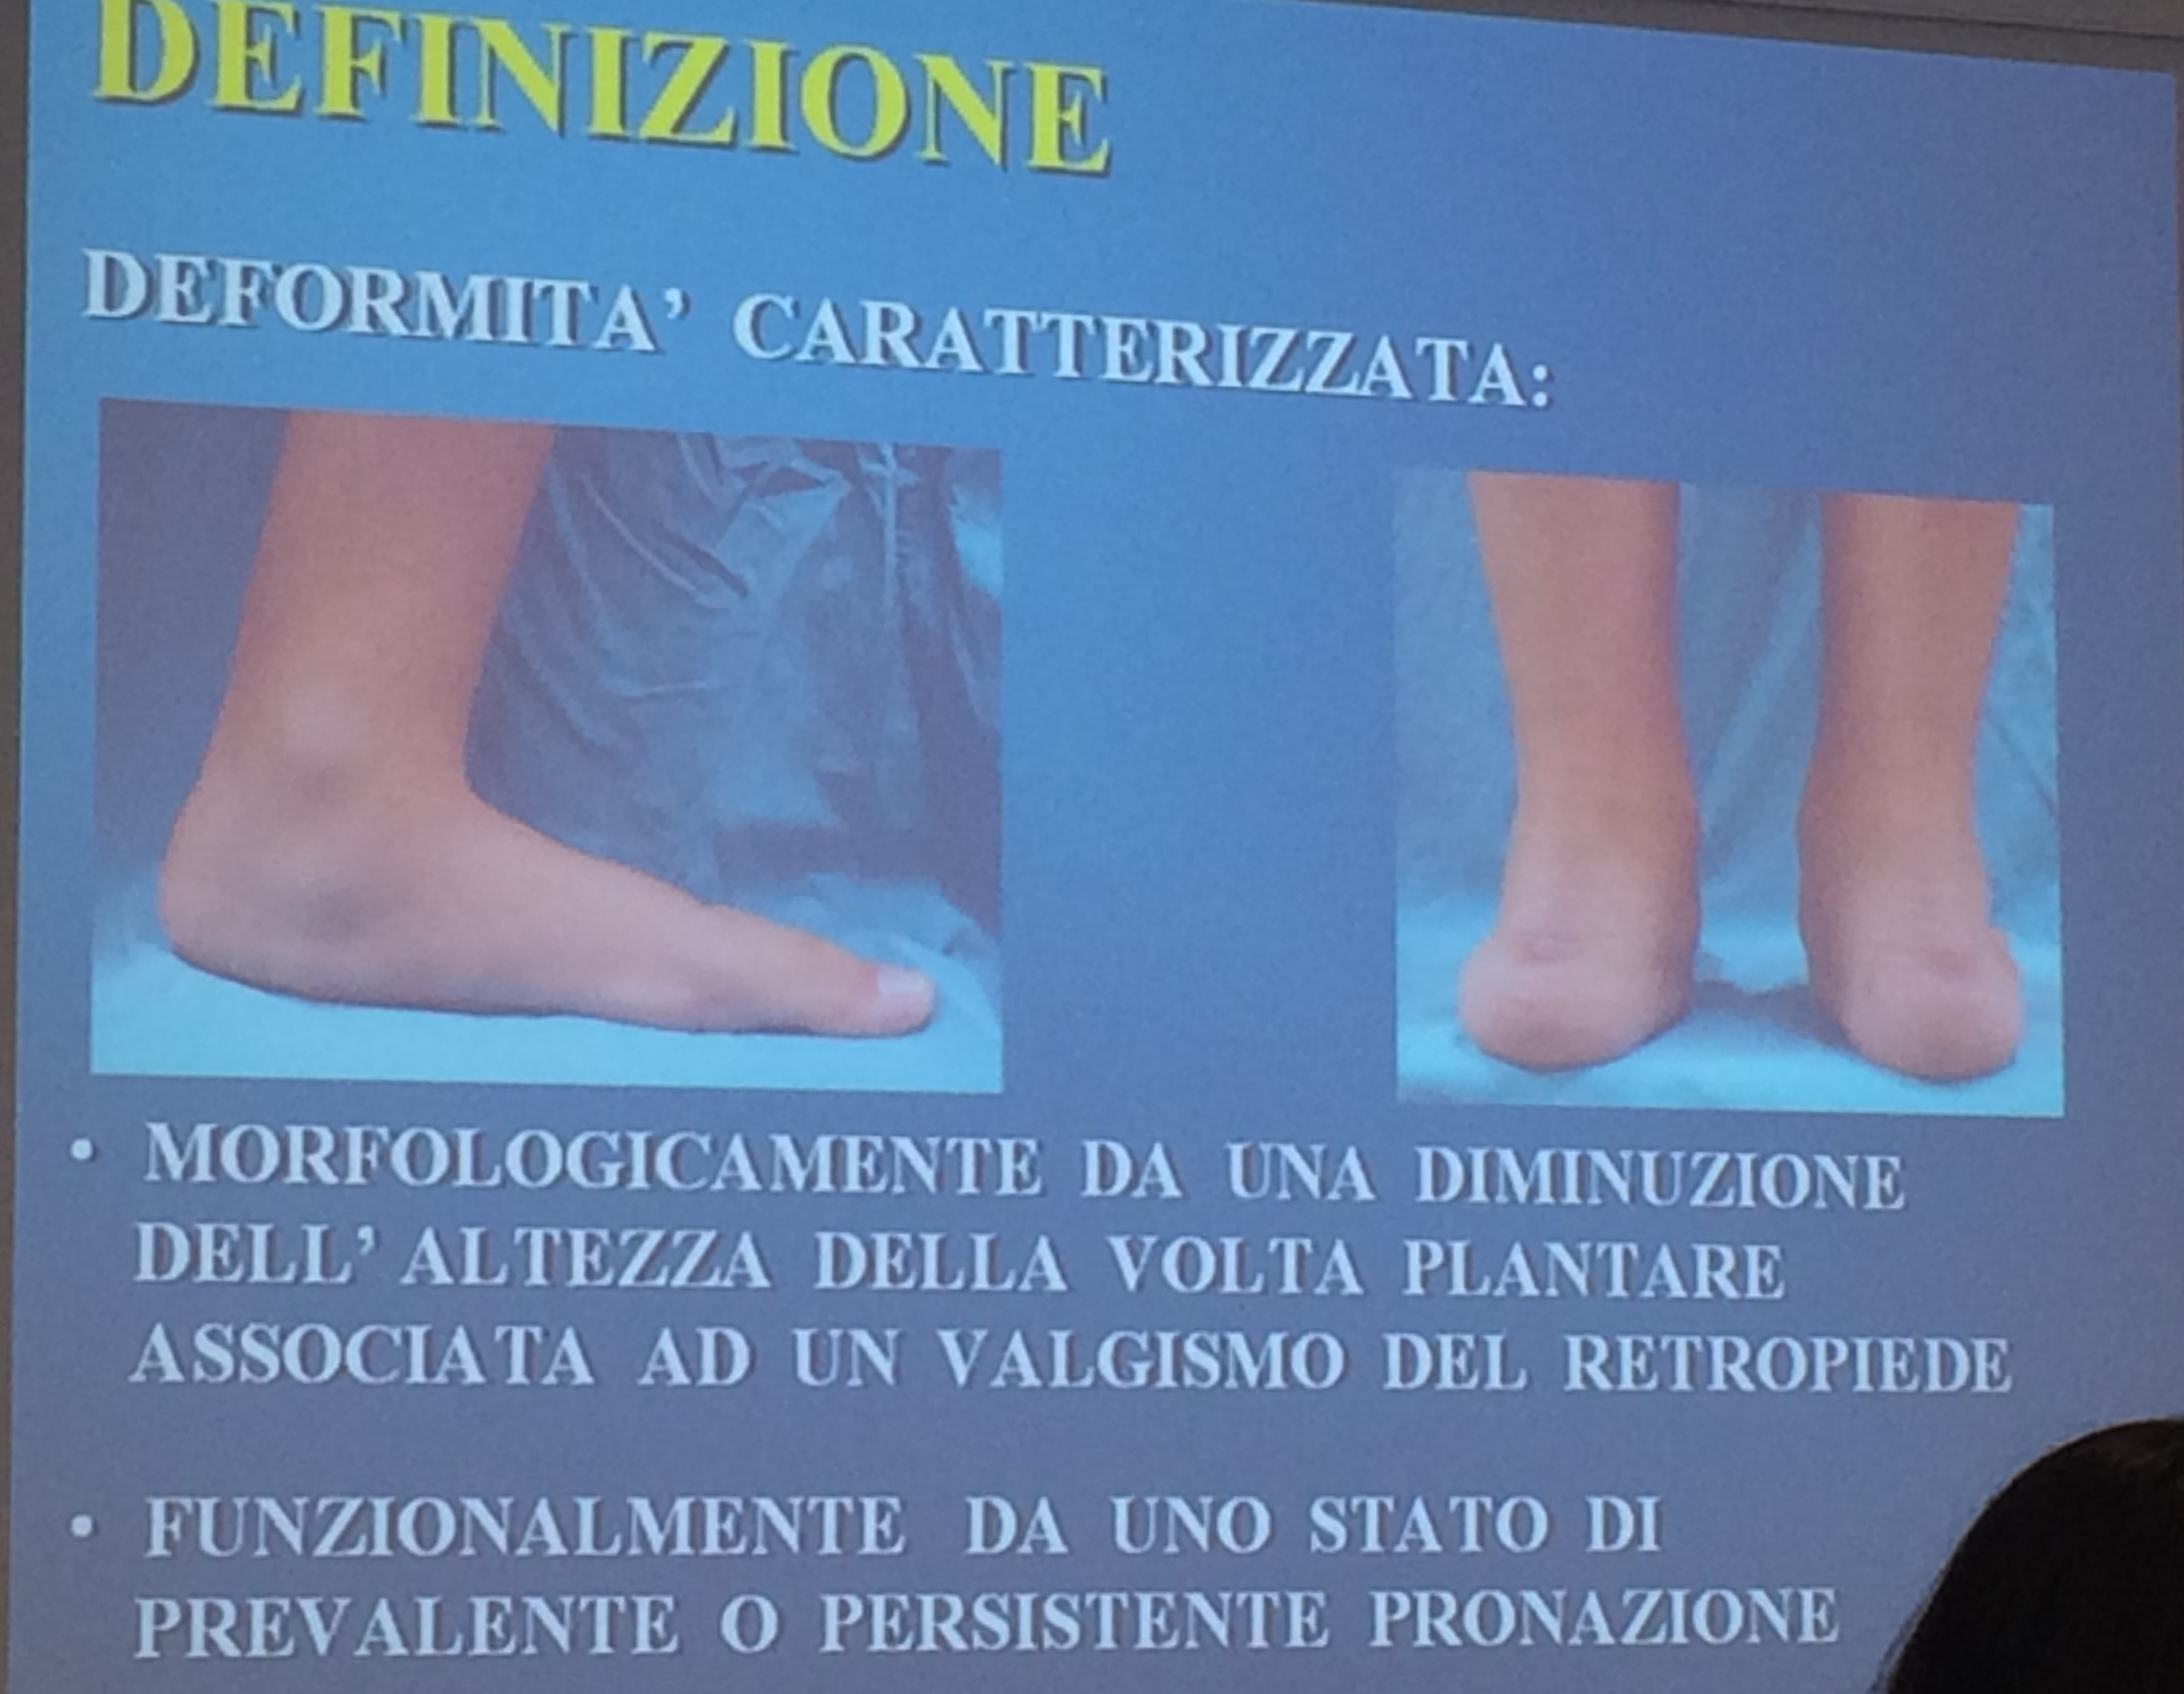
\includegraphics[width=0.4\textwidth]{014/image1.jpeg}
\end{figure}

Il piede piatto è una deformità caratterizzata:

\begin{itemize}
\item
  \emph{Morfologicamente} da una \emph{diminuzione della normale altezza della volta plantare} associata ad un \emph{valgismo del retro piede}. (\emph{Superiore al valore fisiologico di 5\textsuperscript{o}-7\textsuperscript{o})}
\item
  \emph{Funzionalmente} da uno \emph{stato di prevalente o persistente pronazione} \emph{dal momento che il piede non riesce ad alternare questo assetto con quello opposto di supinazione che a sua volta è caratterizzato morfologicamente da un aumento della volta plantare associata a varismo del retro piede.}
\end{itemize}

\textbf{\emph{Il problema non è morfologico bensì funzionale!}}

\subsection{Introduzione}

Negli anni '80 ci sono stati importanti finanziamenti statali per la ricerca nell'ambito della patologia del piede piatto.

Occorre premettere che si osserva comunemente una certa variabilità clinica nei pazienti con piede piatto:

\begin{itemize}
\item
  Soggetti di una certa età con i piedi piatti in cui la deformità è morfologicamente ben evidente, ma non lo è altrettanto da un punto di vista funzionale: non presentano né una sintomatologia patologica né ci sono ripercussioni sulla qualità di vita.
\item
  Soggetti giovani con i piedi piatti in cui, al contrario, morfologicamente la deformità non è molto evidente mentre lo è da un punto di vista funzionale: chiara sintomatologia dolorosa la quale influisce sulla qualità di vita del soggetto.
\end{itemize}

La diagnosi di piedi piatto è relativamente facile: \textbf{\emph{le difficoltà si trovano nel trattamento!}}

I piedi piatti rappresentano una delle principali cause di consultazione ortopedica in età pediatrica.

La ricerca ha portato alla conclusione che il problema dei piedi piatti non è morfologico (come c'è scritto sui libri) bensì \emph{funzionale}.
Il piede normale non è quello bello dal punto di vista morfologico, ma quello che non dà segno di sé dal punto di vista sintomatologico

\subsection{Richiami di anatomia}

\begin{figure}[!ht]
\centering
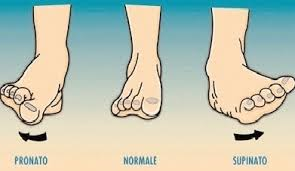
\includegraphics[width=0.4\textwidth]{014/image2.png}
\end{figure}

La conformazione degli elementi scheletrici del piede e i loro rapporti articolari consentono al piede \emph{solo due movimenti complessi triplanari}: (\emph{il prof invita a paragonare il piede ad un elica a passo variabile dove le pale sono avampiede e retropiede)}

\begin{itemize}
\item
  Una \emph{rotazione interna dell'avampiede} e \emph{rotazione esterna del retropiede (calcagno)} che determinano un rilasciamento del piede con riduzione della volta plantare e quindi \textbf{\emph{pronazione.}}
\item
  Una \emph{rotazione esterna dell'avampiede} e \emph{rotazione interna del retropiede (varismo)} che invece determina l'aumento della volta plantare e quindi \textbf{\emph{supinazione}} che è un irrigidimento del piede
\end{itemize}

E' intuitivo che il movimento passivo delle articolazioni è determinato dal movimento attivo muscolare.

La pronazione e la supinazione si alternano in maniera più o meno ritmica per cui il piede si trova in un continuo stato di ``variabilità'' sia in \emph{fase statica} (per esempio quando si è fermi ad osservare uno paesaggio) che nella \emph{fase di spinta} (deambulazione). Durante quest'ultima fase il piede nella \emph{fase iniziale di appoggio a terra} va in \emph{pronazione}: si rilascia e
diventa flessibile non sapendo cosa gli riserva l'ambiente e per questo ha un grande apparato propriocettivo che capta le informazioni utili per l'adattamento (si ricordi l'homunculus sensoriale dove la rappresentazione sensitiva del piede è 10 volte quello della mano).

Nella \emph{fase di spinta} il piede è in \emph{supinazione}: si irrigidisce e trasforma in una struttura rigida (una leva) divenendo l'effettore di una risposta motoria modulata e finalizzata alla realizzazione cinetica di equilibrio e spostamento del corpo.

Le singole articolazioni partecipano al movimento complesso triplanare di pronazione e supinazione in modo armonico e concatenato e costituiscono nel loro insieme un'unità funzionale detta \emph{CATENA CINETICA DEL PIEDE}.

Attraverso l'articolazione tibio-tarsica, la catena cinetica del piede rientra nella più ampia \emph{CATENA CINETICA DELL'ARTO INFERIORE} della quale fanno parte anche caviglia, ginocchio e anca. Infatti ai movimenti di pronazione e supinazione del piede corrispondono movimenti vincolati dell'anca e del ginocchio: \emph{al movimento di pronazione corrisponde la flessione della caviglia, flessione del ginocchio e intra-rotazione dell'anca}. Dati i rapporti reciproche se per esempio dall'esterno riceviamo un insulto meccanico (es. spinta, buca in terra) che determina un impiego del vincolo legamentoso oltre la sua capacità, abbiamo una distorsione: rottura dei legamenti fino alla frattura. (1986)

A proposito di queste relazioni reciproche, il prof. fa riferimento a uno studio americano sul fallimento delle protesi di ginocchio nei casi in cui non era stata eseguita una corretta valutazione della funzionalità del piede. La protesi falliva per cause che partivano da alterazioni della funzionalità del piede: si ha un cedimento della sotto-astragalica ovvero una valgizzazione del calcagno.

\emph{L'alternanza pronazione e supinazione si vede non solo nella fisiologia del piede, ma anche nell'ontogenesi: il bambino nasce con una eccessiva pronazione (piede piatto, ma fisiologico) che poi pian piano durante la crescita diventa normale. Con lo crescita si passa dunque da una condizione di massima pronazione a una di massima supinazione però talvolta si può avere:}

\begin{itemize}
\item
  \emph{Un eccesso di supinazione}
\item
  \emph{Permanenza del piede piatto perché non avviene la supinazione}
\end{itemize}

Come i movimenti del piede sono complessi, anche le sue deformità lo sono e queste possono essere:

\begin{itemize}
\item
  Una \emph{deformità in eccesso di pronazione ovvero il piede piatto}
\item
  Una \emph{deformità in eccesso di supinazione} \emph{ovvero il piede cavo}
\end{itemize}

In entrambi i casi \emph{i movimenti triplanari non si alternano più in maniera ritmica, ma sono fissi} e ciò può essere determinato da alterazioni ossee, capsulo-legamentose o muscolari.

\begin{figure}[!ht]
\centering
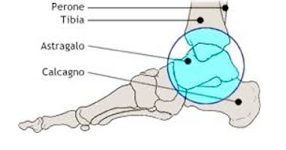
\includegraphics[width=0.4\textwidth]{014/image3.png}
\end{figure}

La definizione quindi non è solo morfologico, ma serve sempre una valutazione di tipo funzionale (\emph{vedi definizione che combina concetto morfologico e funzionale!):} le persone di colore hanno i piedi piatti, ma il calcagno è diritto e la funzionalità del piede è corretta.

L'anatomia patologica è sempre radiografica per quanto riguarda l'ortopedia: la faccia solcata dell'astragalo ci dà un'idea della deformità in pronazione. Ciò si vede dal fatto che il calcagno è più orizzontale (alla vista esterna c'è dunque valgismo) e che l'astragalo rispetto alla tibia è molto più verticale. Normalmente l'angolo tra
l'asse dell'astragalo e l'asse del calcagno è di 110\textsuperscript{o} e nei piedi piatti i gradi di questo angolo sono molti di più.

Aumenta l'asse anche nella proiezione dorso-plantare dove il calcagno tende verso l'esterno e l'astragalo intra-ruota con conseguente crollo della volta plantare. \emph{La rotazione interna dell'astragalo ha anche
un'altra conseguenza: rotazione interna del ginocchio (\emph{si parla di strabismo convergente delle rotule}) e dell'anca da ciò deriva uno stiramento di tutte le parti mediane del piede e della gamba da cui anche il dolore.} Questa situazione è giustificata, come dicevamo, dalla
presenza di una catena cinetica

\begin{figure}[!ht]
\centering
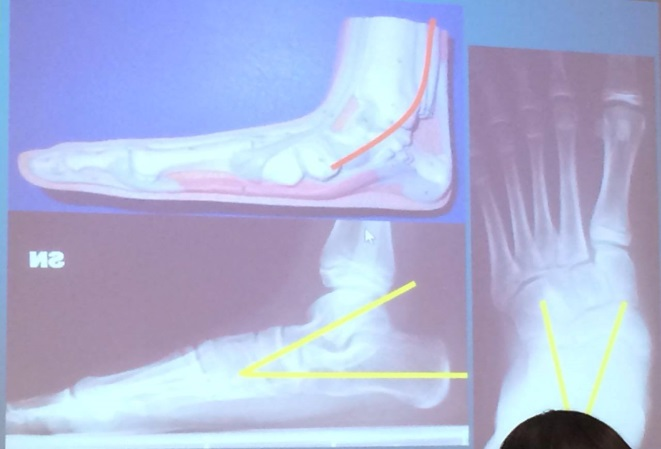
\includegraphics[width=0.4\textwidth]{014/image4.jpeg}
\end{figure}

\begin{figure}[!ht]
\centering
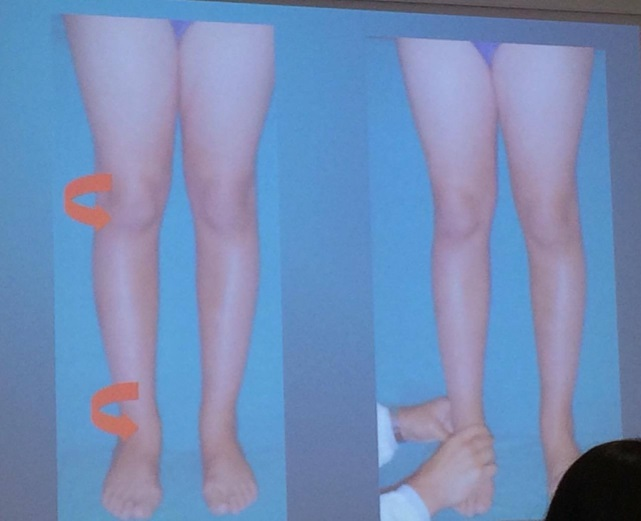
\includegraphics[width=0.4\textwidth]{014/image5.jpeg}
\end{figure}

Dal momento che un piede in pronazione ha la rotula intra-ruotata, correggendo il retro-piede, la rotula si porta in posizione più laterale e corretta.

\subsection{Classificazione Eziologica}

\emph{Deve essere distinto il piede piatto del bambino da quello dell'adulto} perciò possiamo fare una prima classificazione in relazione all'età del paziente:

\begin{itemize}
\item
  Piede piatto dell'infanzia
\item
  Piede piatto dell'adulto (può esordire in età adulta od evolvere dal piede piatto presente nell'infanzia)
\end{itemize}

Per quanto riguarda il piede piatto nell'infanzia, si distingue in:

\begin{itemize}
\item
  \emph{Essenziale} che è quello tipico e più frequente. \emph{Non può essere diagnosticato prima dei 4 anno di età perché prima dei quattro anni il piede piatto è fisiologico}
\item
  \emph{Congenito} che a sua volta può essere associato a:
\begin{itemize}
\item
  \emph{Sinostosi }
\item
  \emph{Ad astragalo verticale }
\end{itemize}
\item
  \emph{Da lassità legamentosa} (es. Sindrome di Ehler-Danlos, Trisomia 21)
\item
  \emph{Esito piede torto congenito equino-varo-supinato} che viene corretto troppo e va in piattismo
\item
  \emph{Neuro-Muscolare (}malattie neurologiche spastiche o flaccide)
\item
  \emph{Forme secondarie ad ipercorrezione del piede torto equino-varo-supinato, ad artrogriposi, a miopatie}
\end{itemize}

Il piede piatto nell'adulto può essere:

\begin{itemize}
\item
  \emph{Reumatico} (per distruzione della membrana sinoviale)
\item
  \emph{Infettivo}
\item
  \emph{Post-traumatico}
\item
  \emph{Diabetico }
\item
  \emph{\emph{Cause di piede piatto nel bambino}}
\end{itemize}

\subsection{Diagnosi}

La classificazione eziologica è fondamentale per un adeguato trattamento. Un'esatta diagnosi si fa con:

\begin{itemize}
\item
  \emph{L'osservazione clinica }
\item
  \emph{Esami strumentali}: non c'è un esame migliore per cui in base al sospetto si ordina Rx, TC, RMN, Elettromiografia.
  
\begin{figure}[!ht]
\centering
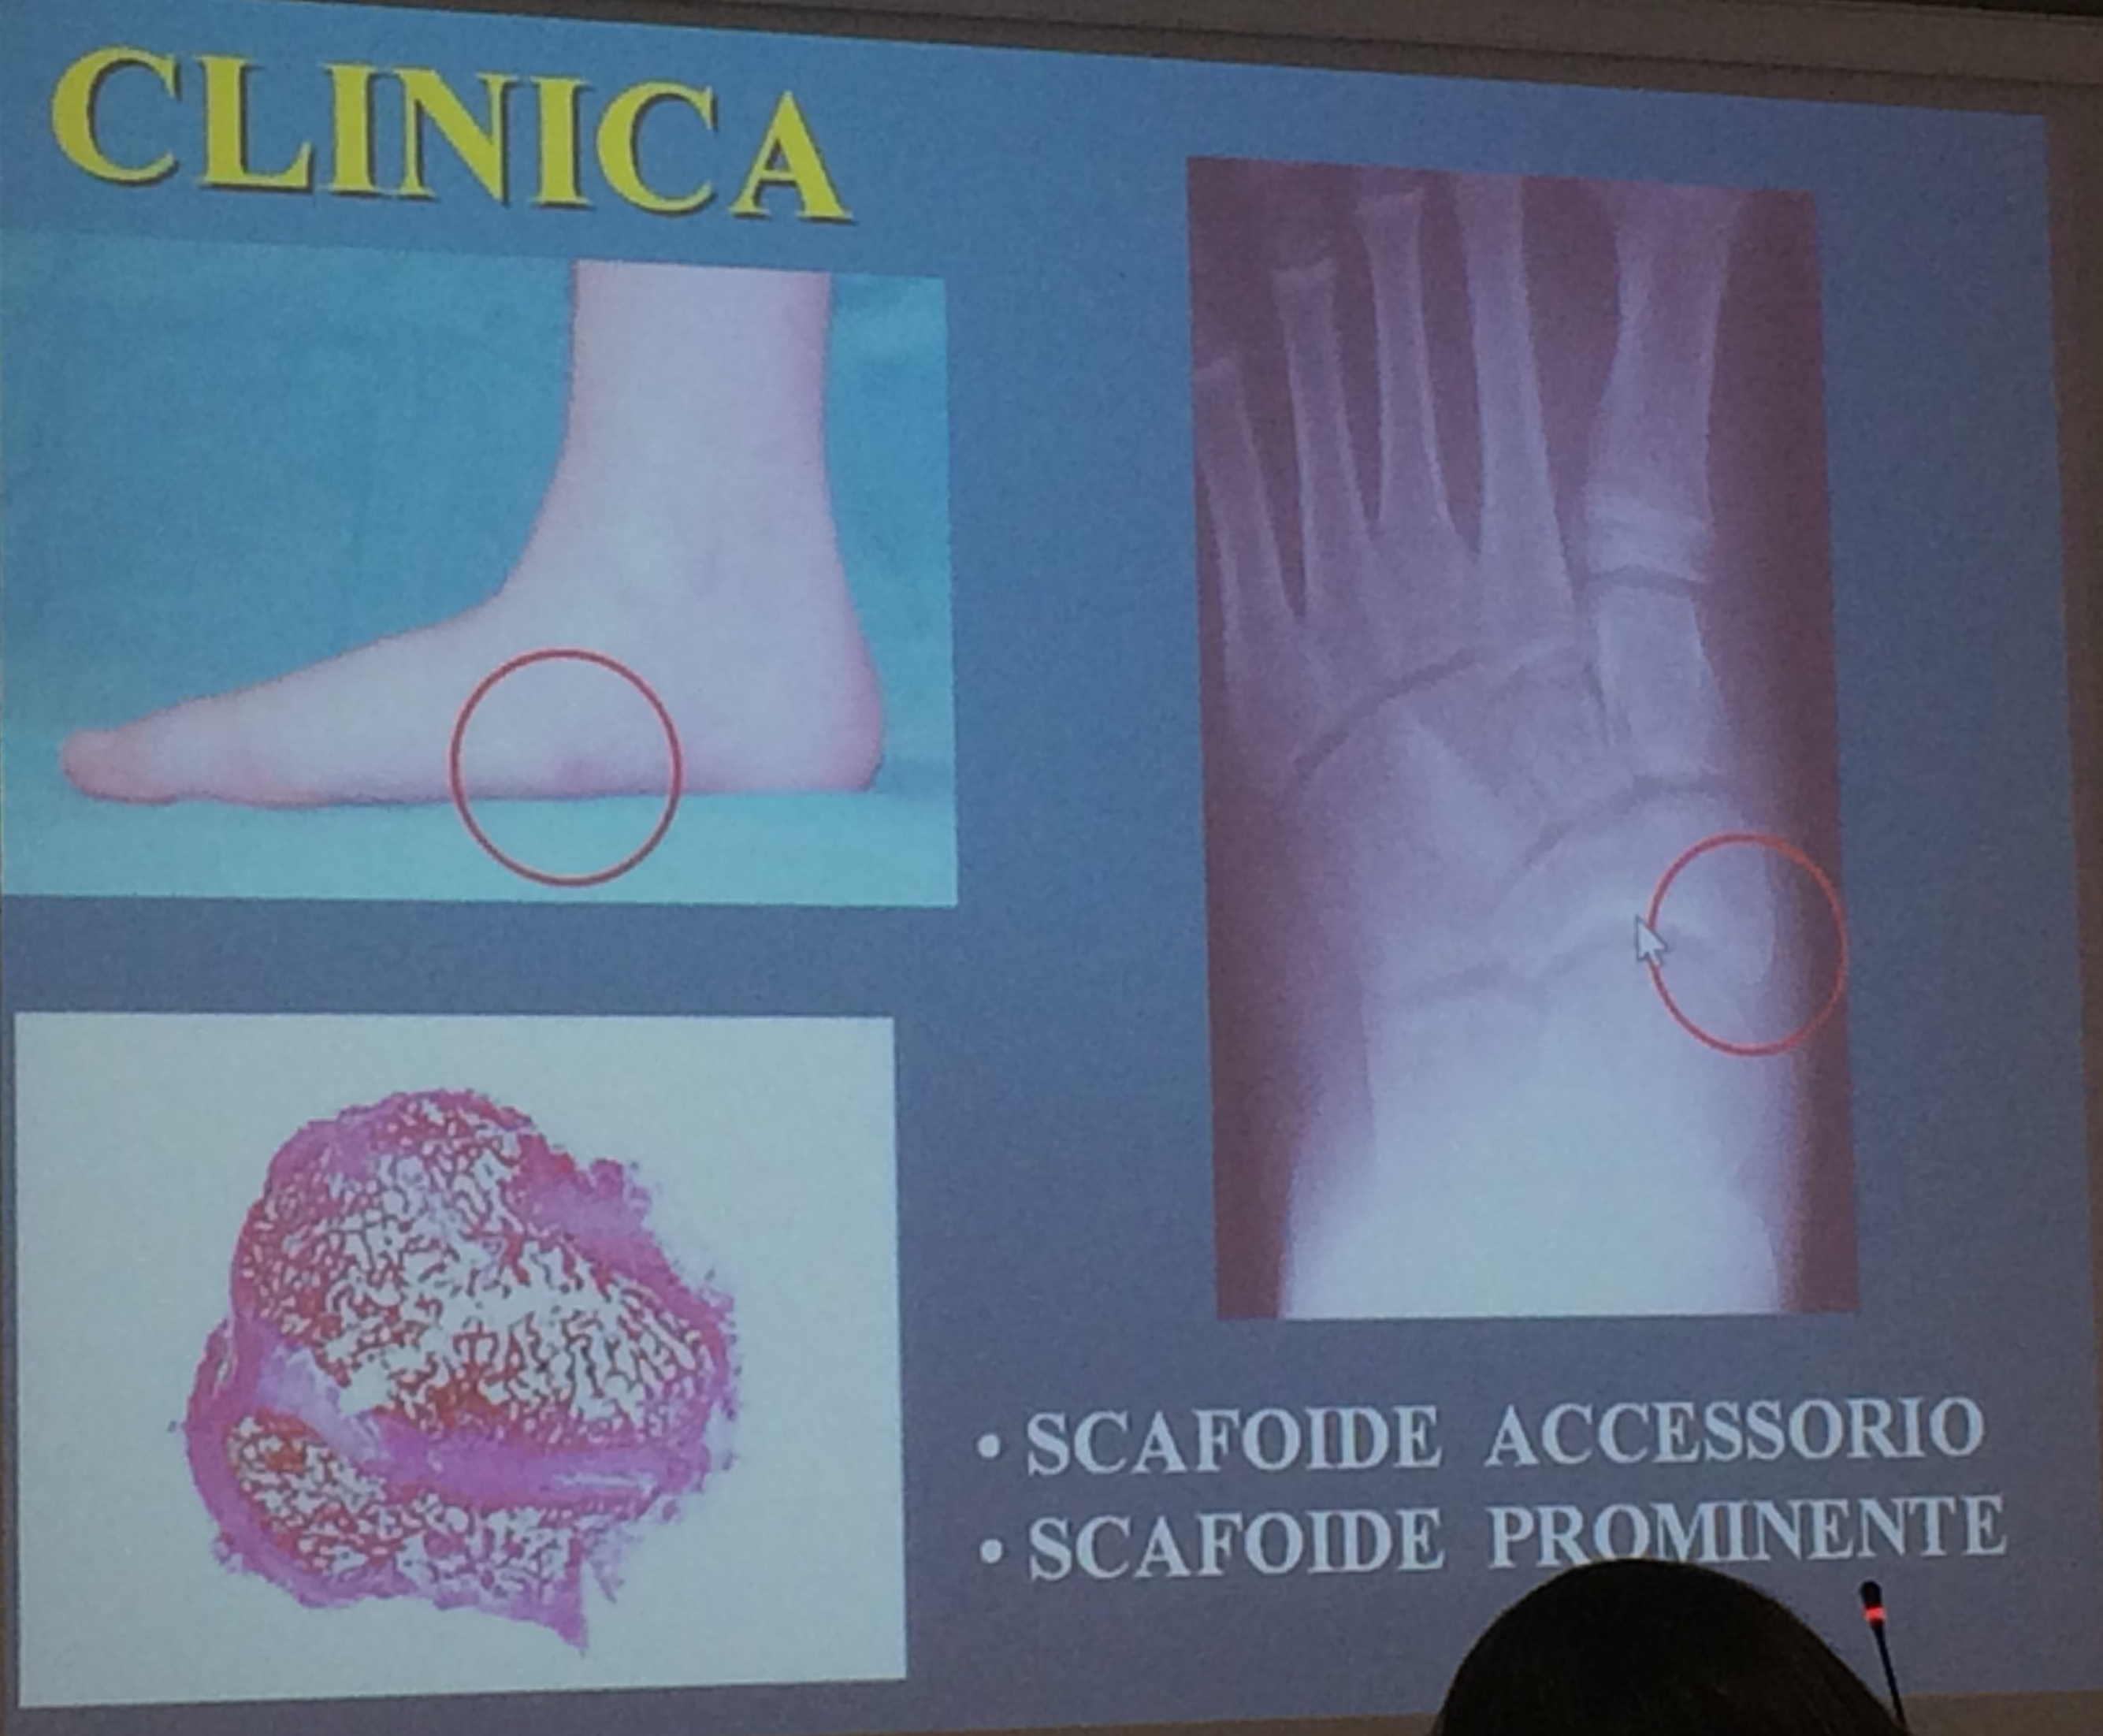
\includegraphics[width=0.4\textwidth]{014/image6.jpeg}
\end{figure}  

L'esame strumentale principale in caso di piede piatto è rappresentato dall'\textbf{esame radiografico} da eseguirsi in \emph{proiezione dorso-plantare} e \emph{latero-laterale}, sempre \emph{sotto carico}. Tipicamente, soprattutto in proiezione dorso-plantare, si mette in evidenza una \emph{rotazione interna dell'astragalo rispetto al calcagno} che a sua volta risulta \emph{ruotato verso l'esterno}, con una aumento dell'angolo individuato dagli assi maggiori di queste due ossa. Sempre in queste proiezione può talvolta essere messa in luce la presenza di uno \textbf{scafoide accessorio} a livello dell'inserzione del tibiale posteriore. La proiezione latero-laterale, invece, mostra la posizione più orizzontale del calcagno e la caduta in basso della testa dell'astragalo con riduzione della volta plantare. La TC ha un uso limitato nel piede piatto, essendo in genere riservata solo per evidenziare eventuali sinostosi astragalo-calcaneari o calcaneo-scafoidea.
\item
  \emph{Esame funzionale} \emph{attraverso manovre standardizzate} che permettono di capire se un piede è funzionalmente piatto o lo è solo morfologicamente
\end{itemize}

L'insieme di queste tre componenti ci permette di eseguire una corretta diagnosi e di indirizzare il paziente verso il trattamento migliore che potrà essere:

\begin{itemize}
\item[1.]
  Chirurgico
\item[2.]
  Riabilitativo
\item[3.]
  Ortesico
\end{itemize}

\subsection{Piede piatto idiopatico o essenziale}

Il passaggio tra pronazione e supinazione è presente anche nella filogenesi (evoluzione della specie) e nell'ontogenesi (evoluzione dell'individuo).

Nelle varie settimane di \textbf{\emph{sviluppo fetale}} abbiamo un \textbf{\emph{progressivo passaggio da pronazione a supinazione e poi di nuovo pronazione}} (da cui l'ipotesi che il piede equino-varo-supinato sia dovuto a un arresto durante lo sviluppo fetale).

Nel \textbf{\emph{periodo perinatale}} (dalla nascita fino ai 4 anni di età) abbiamo un \textbf{\emph{eccesso di pronazione}} quindi fino a questa età il piede piatto è fisiologico (l'utilizzo di plantari è totalmente inutile).

\textbf{\emph{Dopo i 4 anni}}, sotto gli stimoli dell'ambiente esterno, il piede \textbf{\emph{si sviluppa con passaggio graduale verso la supinazione e il piede raggiunge la sua morfologia definitiva}} e se in questa fase qualcosa non va allora si interviene.

\textbf{\emph{Si può propriamente parlare di piede piatto essenziale o idiopatico solo dopo i 4 anni di età}} in quanto prima di questa età il piede piatto dei bambini è da considerarsi parafisiologico: rappresenta una fase dello sviluppo morfologico del piede.

\subsubsection{Clinica}

(Il difetto è sempre lo stesso! Descritto nella parte precedente)

Il \emph{sintomo principale} è rappresentato dal dolore o meglio dal \emph{fastidio}. Può essere \emph{a livello del collo del piede, del ginocchio, del tendine di Achille o dei peronei}. Normalmente il fastidio compare attorno ai dieci anni e può essere dovuto a:

\begin{itemize}
\item
  Rapido accrescimento e conseguentemente rapido incremento di peso
\item
  Inizio di un attività sportiva più intensa
\end{itemize}

All'\emph{esame obiettivo} possiamo osservare:

\begin{itemize}
\item
  \emph{Riduzione della volta plantare con rotazione esterna del tallone.}
\item
  Ci può essere un \emph{arrossamento nella zona medio-mediale del piede} per un eccessivo carico soprattutto se si ha uno scafoide accessorio (piccolo osso soprannumerario) dove si attacca il tendine del tibiale posteriore (quello che irrigidisce il piede e sostiene la volta portandolo in supinazione).
\end{itemize}

La presenza dello scafoide accessorio indica una situazione in cui il tendine del tibiale posteriore ``tira meno'' e in cui il piede è dunque continuamente pronato. La stessa condizione si può avere nel caso dello ``Scafoide prominente''.

\textbf{\emph{Quindi l'esame clinico deve valutare non solo se un piede è morfologicamente piatto ma se lo è anche funzionalmente piatto.}}

La differenza tra il piede piatto asintomatico e quello sintomatico sta nella funzione perciò solo quando il piede nel bambino è funzionalmente piatto verrà trattato {[}trattamento del piede piatto nella prossima lezione{]}.

\subsubsection{Complicanze del piede piatto essenziale}

Diverse complicanze sono associate al piede piatto essenziale e tutto sono dovute all'eccesso di pronazione:

\begin{itemize}
\item
  \emph{La sindrome da pronazione cronica. (La più comune!!)} In una condizione di eccesso di pronazione (appunto pronazione cronica) il tibiale posteriore non si riposa mai ed il risultato è un'infiammazione del tendine. In generale, a causa di questa mancata alternanza tra pronazione e supinazione, le strutture capsulo-legamentose, tendinee, muscolari e vascolo-nervose mediali sono sottoposte ad una distensione continua senza adeguate pause di riposo e ciò determina la comparsa di dolore. Il dolore da pronazione cronica si localizza non solo a livello del retro piede, ma anche a livello del tendine di Achille, dei tendini peronei e dell'inserzione del tibiale posteriore sullo scafoide così come a livello della caviglia e talvolta anche del ginocchio. I fattori che influenzano l'entità della sintomatologia dolorosa sono essenzialmente due: l'\emph{importanza del deficit funzionale} ed il \emph{carico di lavoro del piede}. Da ciò deriva quindi che un piede piatto infantile, piuttosto elastico e mobile, risulta scarsamente dolente all'inizio, ma con l'andare del tempo (in genere a partire dei 9-10 anni) i sintomi si intensificano e diventano più frequenti, soprattutto quando la massa corporea tende ad aumentare ed il soggetto svolge attività fisica più intensa.
\emph{La gran parte della patologia del piede è determinato dall'eccesso
di pronazione o supinazione.}

\item
  L'eccesso di pronazione del retropiede determina una deformità articolare. Questa condiziona un allargamento del ventaglio metatarsale (spazio tra 1\textsuperscript{o} e 2\textsuperscript{o} metatarso) e quindi, \emph{per un gioco muscolare, la deviazione dell'alluce e la formazione dell'alluce \emph{valgo} detto biomeccanico.}

Se una ragazza di 18 anni si presenta con i piedi piatti e l'alluce valgo, operarla per l'alluce valgo è inutile perché dopo qualche anno si ripresenta dal momento che non viene corretta la causa. Nell'alluce valgo il dito tende a storcersi in pronazione e a correggersi in supinazione. Se si corregge il piede piatto, si corregge anche l'alluce valgo.

\item
  La pronazione del retropiede fa sì che il primo metatarsale sia sollevato e appoggi meno rispetto agli altro così da sovraccaricare sul secondo e terzo metatarsale. (Il primo metatarsi non ``cade'' semmai ``vola'' perché non poggia) Ciò determina un'ischemia nella zona costantemente compressa e la cute reagisce portando alla formazione del callo (togliere un callo non serve a niente, in quanto è un meccanismo di compenso al carico che la cute adotta).
N.B. L'alternanza pronazione-supinazione è necessaria per il riposo delle strutture

\begin{figure}[!ht]
\centering
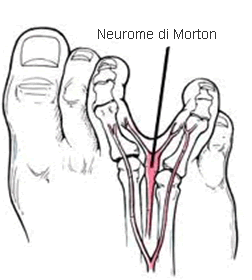
\includegraphics[width=0.4\textwidth]{014/image7.png}
\end{figure}

\item 
  Si ha \emph{insufficienza del primo metatarso} e metatarsalgia. Il sovraccarico delle teste metatarsali comporta anche uno squilibrio muscolare a livello dei muscoli ad azione sulle dita e quindi la comparsa delle deformità ``griffe delle dita''.

\item
  \emph{Neuroma di Morton:} tumore benigno, ma dolorosissimo e complicato perché si forma nel ramo anastomotico sensitivo che va ad innervare i margini contrapposti del terzo e del quarto dito. Questo ramo passando sotto al legamento inter-metatarsale, in condizioni di pronazione, va a contatto con il legamento. Nel tempo si forma un pallino (il neuroma) che determina una compressione del nervo ed evoca una sintomatologia dolorosa improvvisa (definita ``Malattia delle vetrine'' poiché l'uso delle scarpe peggiora il dolore e il paziente finge di guardare le vetrine per dare in realtà una tregua al dolore. Comune negli autisti e ciclisti!).

\item
  \emph{Tenovaginite/ Peritendinite:} infiammazione del tibiale posteriore perché non si riposa mai a causa dell'eccesso pronazione.

\item
  \emph{Sindrome del tunnel tarsale} conseguente alla pronazione cronica con stiramento del nervo tibiale posteriore. Si risolve facilmente con un plantare che riporti il tallone in posizione.

\item
  \emph{Fascite plantare}: riduzione della volta plantare. L'aponeurosi plantare viene stirata progressivamente (trazione eccessiva) e si ha una flogosi che porta poi alla formazione di speroni postero-inferiori (\emph{metaplasia ossea}).

\item
  Anche le articolazioni sono coinvolte dal momento che non si riposano mai e in tal senso si può avere lo sviluppo di gravi \emph{artrosi}: \emph{\emph{piede piatto artrosico}}, rigido e non più correggibili.

\item
  \emph{Alterazioni da usura delle \emph{articolazioni capsulo-legamentose e tendinee mediali}: in alcuni casi il tendine del tibiale posteriore, a causa della sua porzione al di sotto del malleolo interno, può andare incontro anche ad allungamento o improvvisa rottura con aggravamento della deformità del piede. }

\item
  Non è infrequente la formazione di vene varicose in questo caso perché manca la spinta a tergo sul Sangue da parte della \emph{soletta venosa di Lejars} e supinazione e quindi si ha stasi venosa.
\end{itemize}

\emph{Per evitare l'insorgere di queste complicanze nell'adulto è necessario un \emph{adeguato trattamento in fase di accrescimento}, che naturalmente dovrà essere la \textbf{\emph{conseguenza di un'attenta valutazione che permetta di distinguere un piede morfologicamente piatto
da un piede ``funzionalmente'' piatto.}}}

\subsubsection{Test funzionali e complementari}

\emph{Da quanto detto sopra è assolutamente evidente che la morfologia non è sufficiente per tipizzazione un piede piatto infatti per fare questa è necessaria un'analisi della funzione. Bisogna infatti valutare se quel piede morfologicamente piatto riesce ad alterare o meno la pronazione e la supinazione oppure se prevale la pronazione. Infatti solo il deficit funzionale giustifica il trattamento. Vediamo quindi quali sono le prove necessarie per capire se un piede è solo morfologicamente piatto oppure lo è anche funzionalmente:}

\begin{itemize}
\item
  Il piede funzionalmente piatto ha una \emph{difficoltà a mantenere l'equilibro in stazione monopodalica} (su un piede solo senza appoggiarsi). \emph{Il piede funzionalmente piatto non riesce ad alternare pronazione e supinazione per cui il soggetto, in posizione monopodica, non riuscirà a mantenere l'equilibrio su un piede solo.}
\item
  Il paziente affetto da piedi piatti ha \emph{scarsa correggibilità in stazione eretta} ad esempio chiedendo di camminare sulla parte esterna del piede, recluta il muscolo estensore dell'alluce, il quale è un supinatore perché muscolo mediale, poiché il muscolo tibiale esterno è insufficiente e non riescono a supinare.
\item
  Se chiediamo di \emph{camminare in punta di piedi} mentre un soggetto normale ha il tallone che intra-ruotano (varizzano) perché il flessore dell'alluce passa sotto il sustentaculum tali. In un paziente con il piede funzionalmente piatto rimane valgo (intra-ruotato). \emph{Nel soggetto con piede piatto morfologico (e non funzionale) si osserva una correzione del valgismo del calcagno che invece non si osserva nel piede piatto funzionale}

\begin{figure}[!ht]
\centering
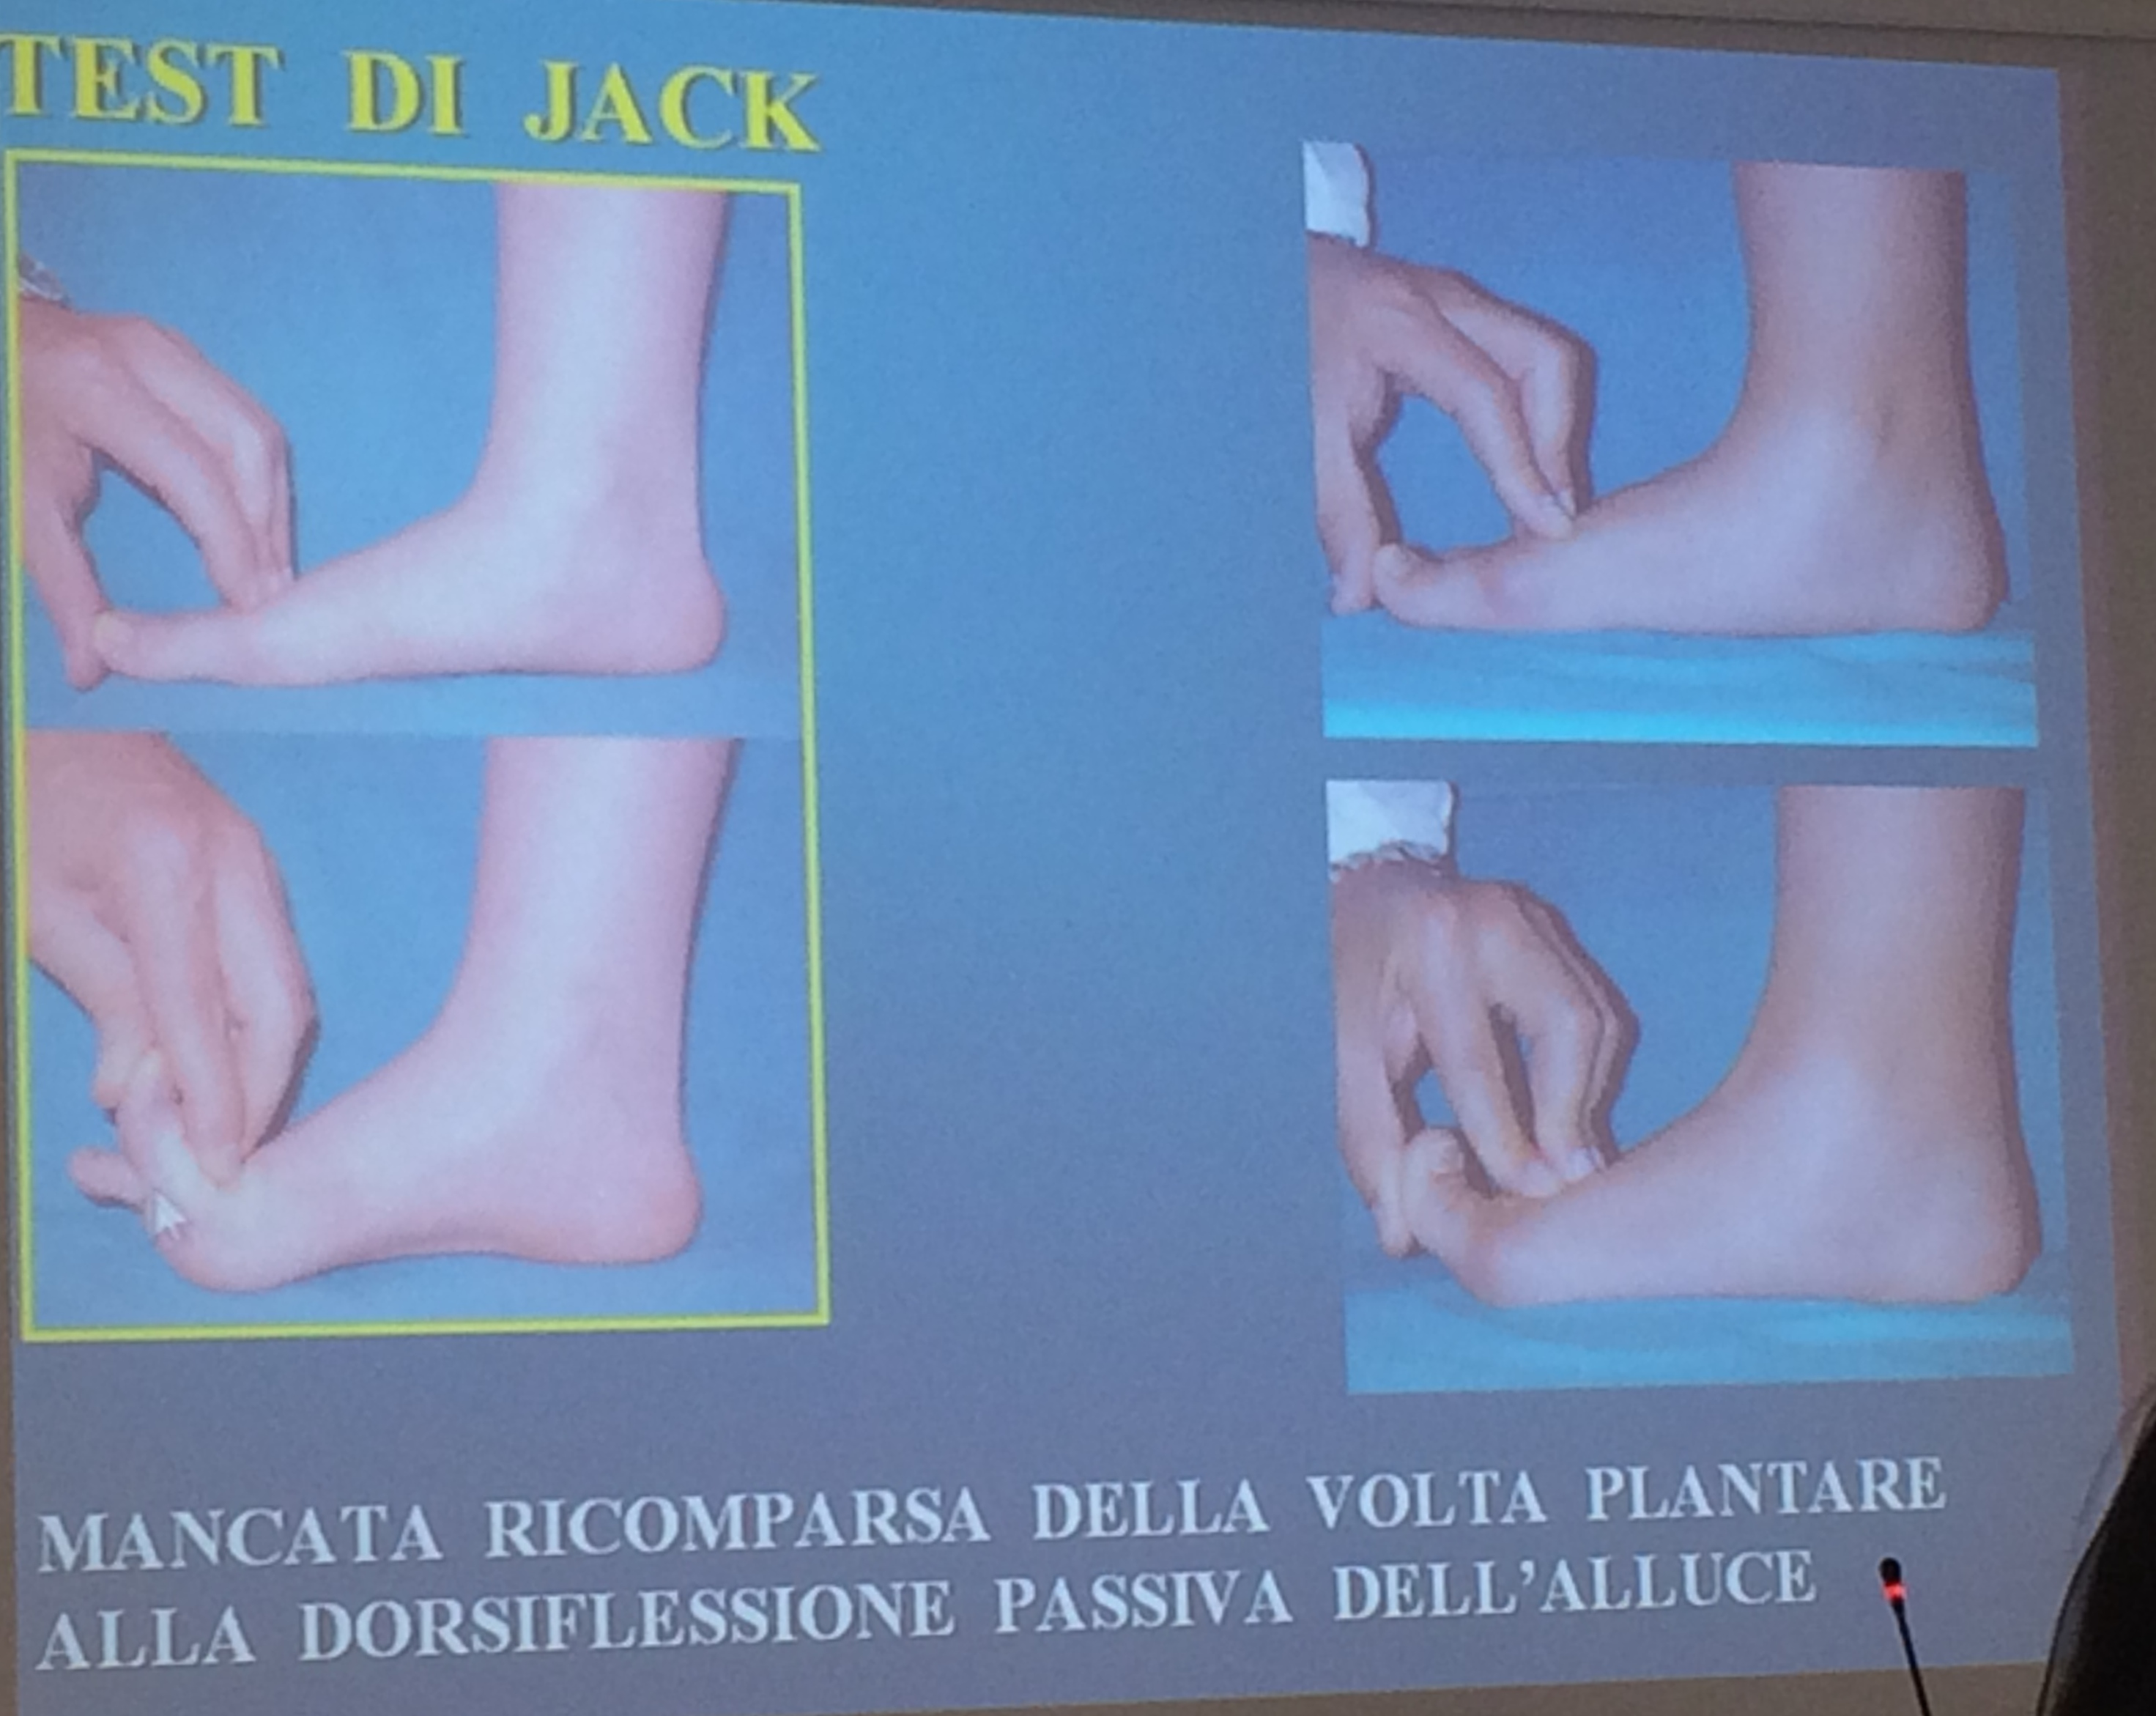
\includegraphics[width=0.4\textwidth]{014/image8.jpeg}
\end{figure}
  
\item
  Nell'immagine è esemplificato il \emph{test di Jack}: mancata ricomparsa della volta plantare alla dorsiflessione passiva dell'alluce da parte dell'esaminatore.
\item
  \emph{Difficoltà in stazione eretta a deambulare sui talloni} (retrazione del sistema tricipite-tendine di Achille).
\item
  \emph{Test di Silfverskiold}: usato in molti ambiti. Se c'è un piede piatto, si ha una limitazione della dorsi-flessione passiva del piede dopo correzione manuale della deformità. Il tricipite è un muscolo bi-articolare e, se io induco un movimento di supinazione a ginocchio esteso, il tendine di Achille ruota e il piede non va oltre l'angolo retto per una maggiore tensione dei m. gemelli. (Importante non solo in diagnosi, ma anche nel trattamento chirurgico perché è necessario in questo caso allungare anche il tendine di Achille.) Nel bambino questa situazione si manifesta con la scarsa alternanza tra pronazione e supinazione; le strutture quindi non si riposano ed evocano dolore (``discomfort''). Si associa ad un mancato movimento del bambino e a tutto ciò che consegue dal punto di vista psicologico. Questi disturbi (dolore alla caviglia, ginocchia, piede, tallone) compaiono a circa 10 anni, in concomitanza con: aumento di peso, crescita corporea, inizio di attività sportive, tutte situazioni che determinano un aumento dello stress sulle strutture osteo-articolari.
\end{itemize}

\subsection{Piede piatto congenito}

Sono tutti piedi \emph{funzionalmente piatti} perché \emph{rigidi}.
Distinguiamo:

\begin{itemize}
\item
  \emph{Piede piatto congenito associato a sinostosi}: mancata segmentazione più che fusione fibrosa, cartilaginea od ossea (più o meno estesa) fra astragalo e calcagno o fra calcagno e scafoide che può essere associata o meno a deformità in piattismo. In questo caso un trattamento identico a quello del piede piatto essenziale porta ad un fallimento totale. L'eziologia di questa condizione è ancora dubbia, ma si pensa sia un difetto di segmentazione del mesenchima primitivo (Harris, 1955). Dal punto di vista clinico non cambia niente rispetto al piede piatto essenziale. \emph{Si presenta come un piede piatto rigido (per cui il plantare è inutile) \emph{e spesso deformato}.} Rigidità e deformazione determinano un riduzione della motilità attiva e passiva in prono-supinazione con contrattura dei peronei (che concorre alla rigidità insieme alla formazione della barra) per un probabile adattamento alla sinostosi. Quindi avremo insufficienza funzionale e comparsa dei dolori (tra 12-16 anni) in concomitanza con l'ossificazione della barra \emph{che nasce cartilaginea e pian piano diventa ossifica e ciò determina rigidità e insufficienza funzionale. Talvolta si parla anche di piede piatto contratto perché c'è una contrattura involontaria dei peronei e degli estensori}
\emph{N.B. Si possono avere barre senza piedi piatti, ma è raro.}

\begin{figure}[!ht]
\centering
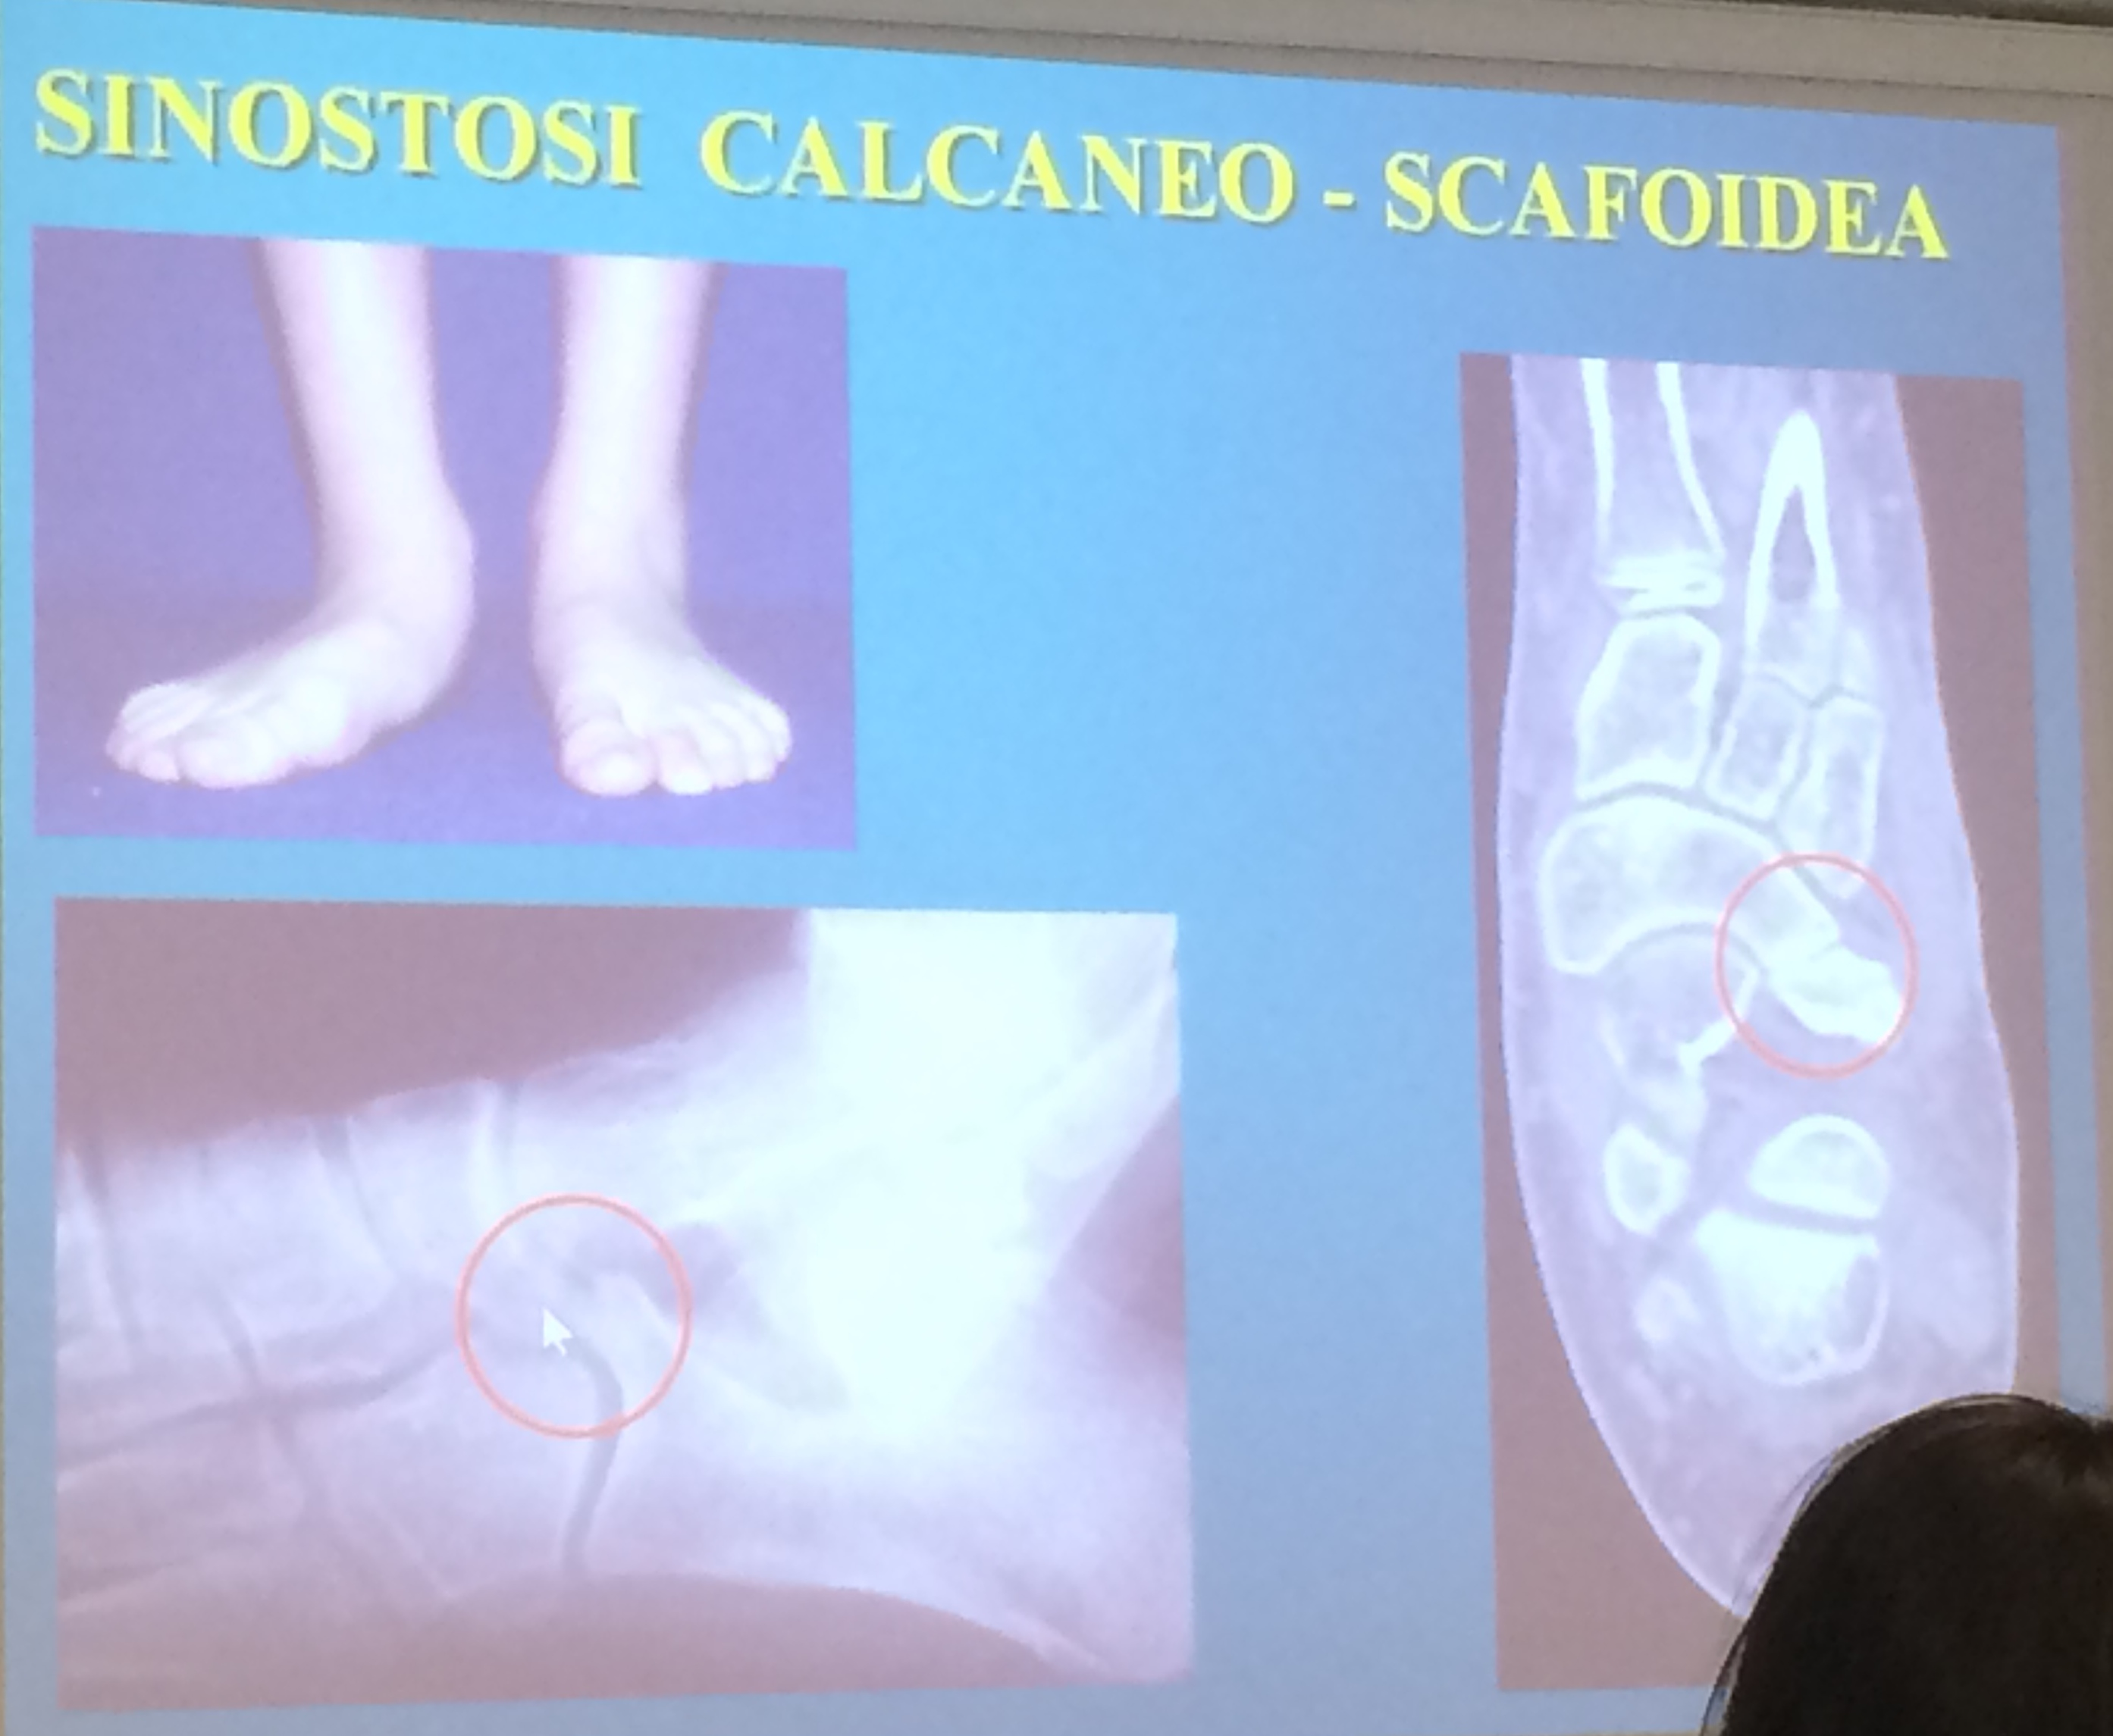
\includegraphics[width=0.4\textwidth]{014/image9.jpeg}
\end{figure}

\item
  \textbf{Piede piatto congenito associato a astragalo verticale:} forma particolare di piede piatto congenito caratterizzato da una lussazione o sub-lussazione dell'articolazione astragalo scafoidea; a \emph{seguito di un errore genetico quel processo di ``caduta'' dell'astragalo, che si ha anche nella forma idiopatica, è estremizzato.} Presenta il caratteristico ``piede a dondolo'' dove il calcagno non tocca in terra con torsione della volta plantare. E' caratterizzato da evidenti malformazioni:
\begin{itemize}
\item
  Estrema rigidità
\item
  Retrazione del tendine di Achille e dei tendini peronei.
\item
  Si può associare anche ad una adduzione dell'avampiede (``piede a z congenito'')
\end{itemize}
\end{itemize}

\begin{figure}[!ht]
\centering
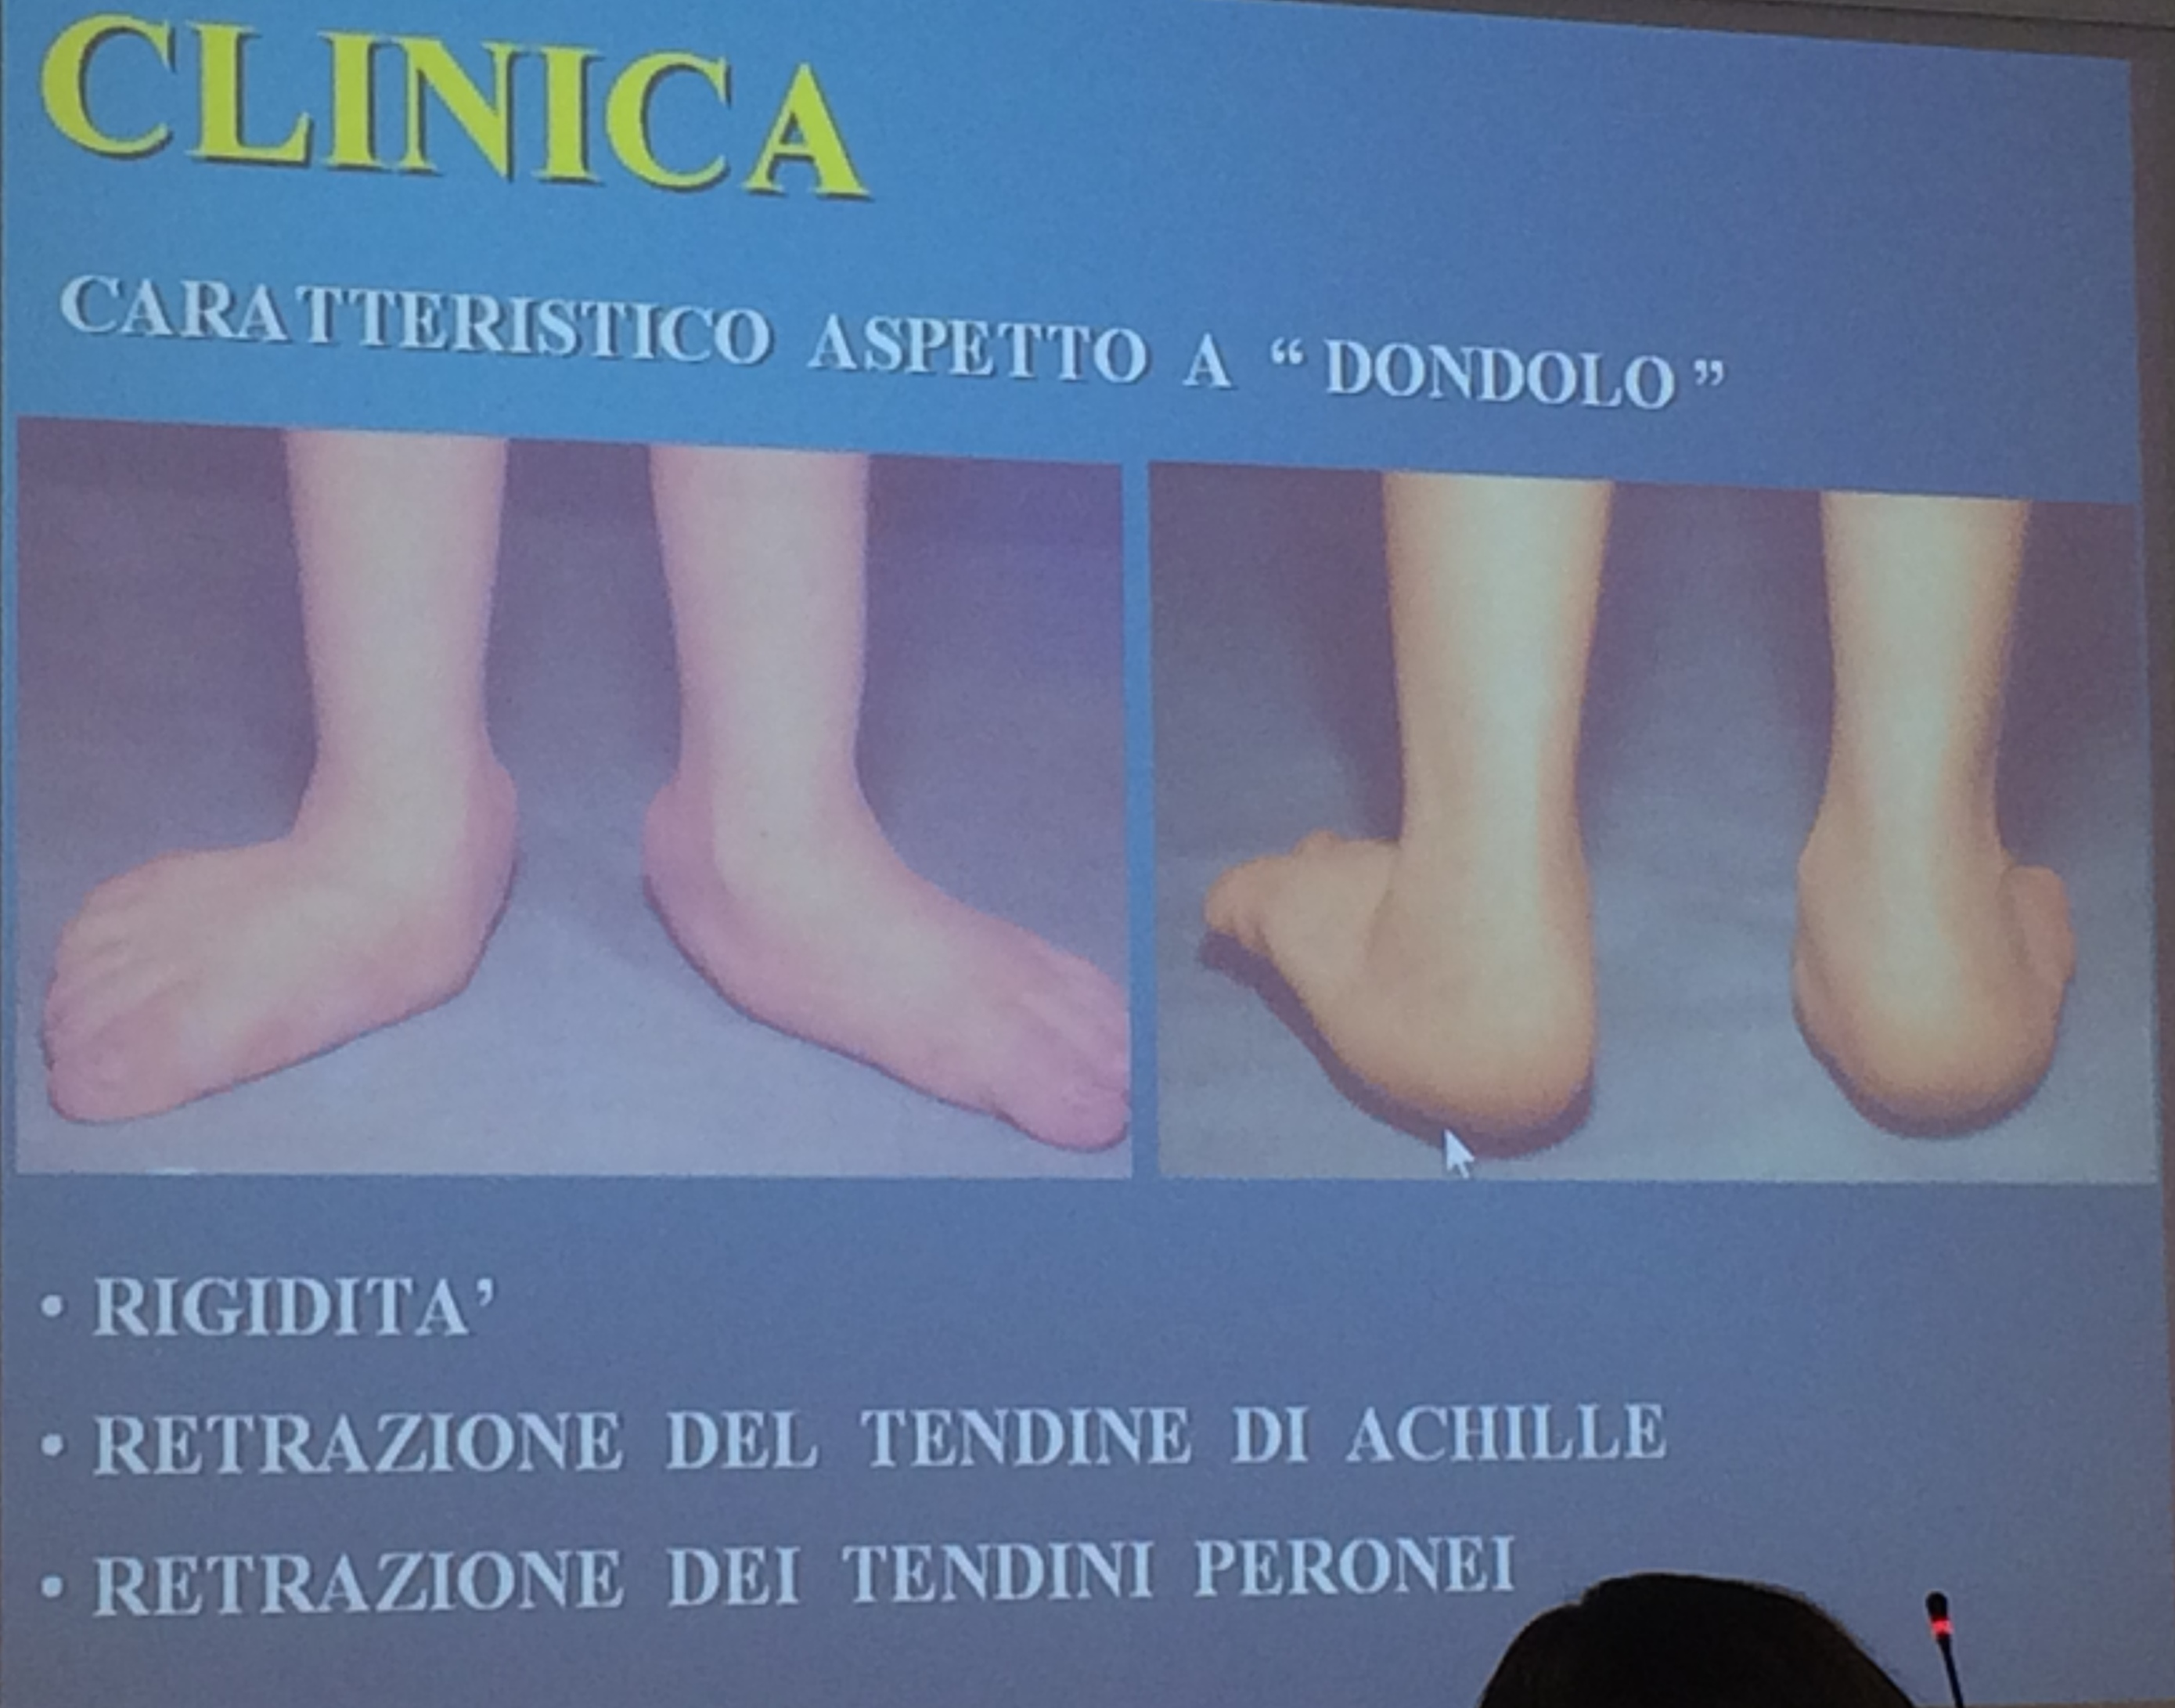
\includegraphics[width=0.4\textwidth]{014/image10.jpeg}
\end{figure}

\begin{figure}[!ht]
\centering
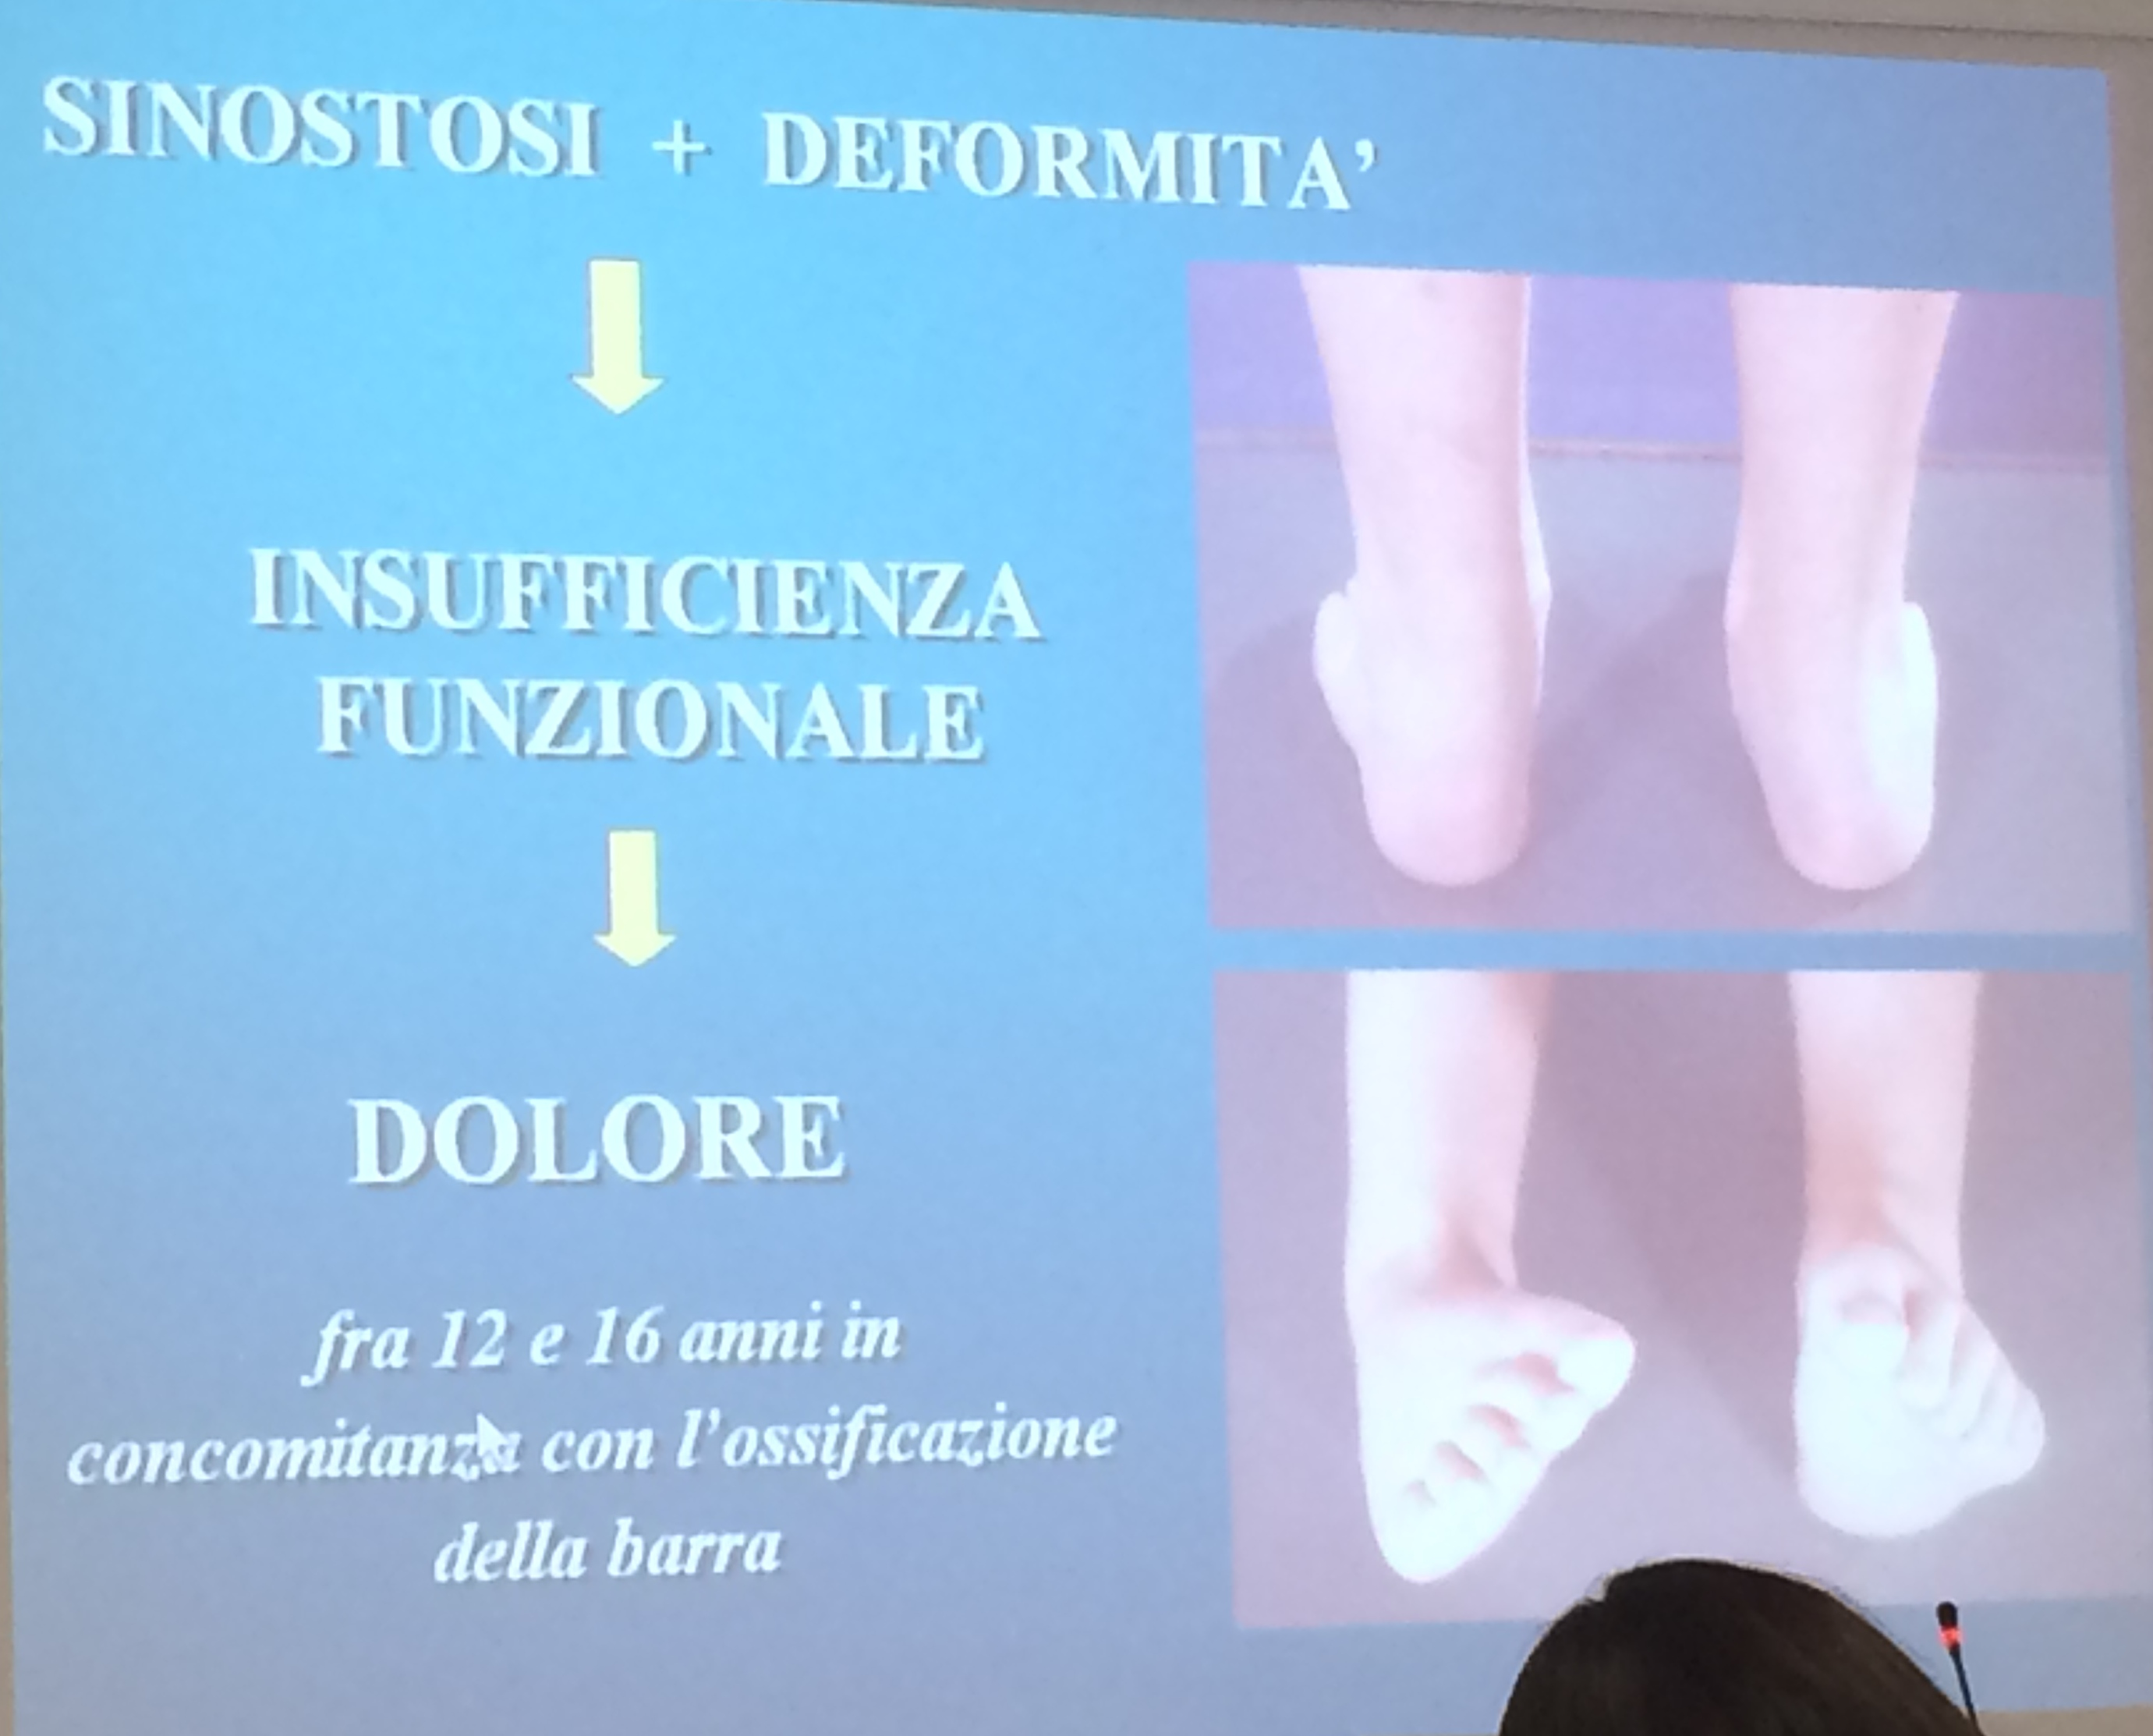
\includegraphics[width=0.4\textwidth]{014/image11.jpeg}
\end{figure}

\subsection{Piede piatto neuro-muscolare}

\begin{figure}[!ht]
\centering
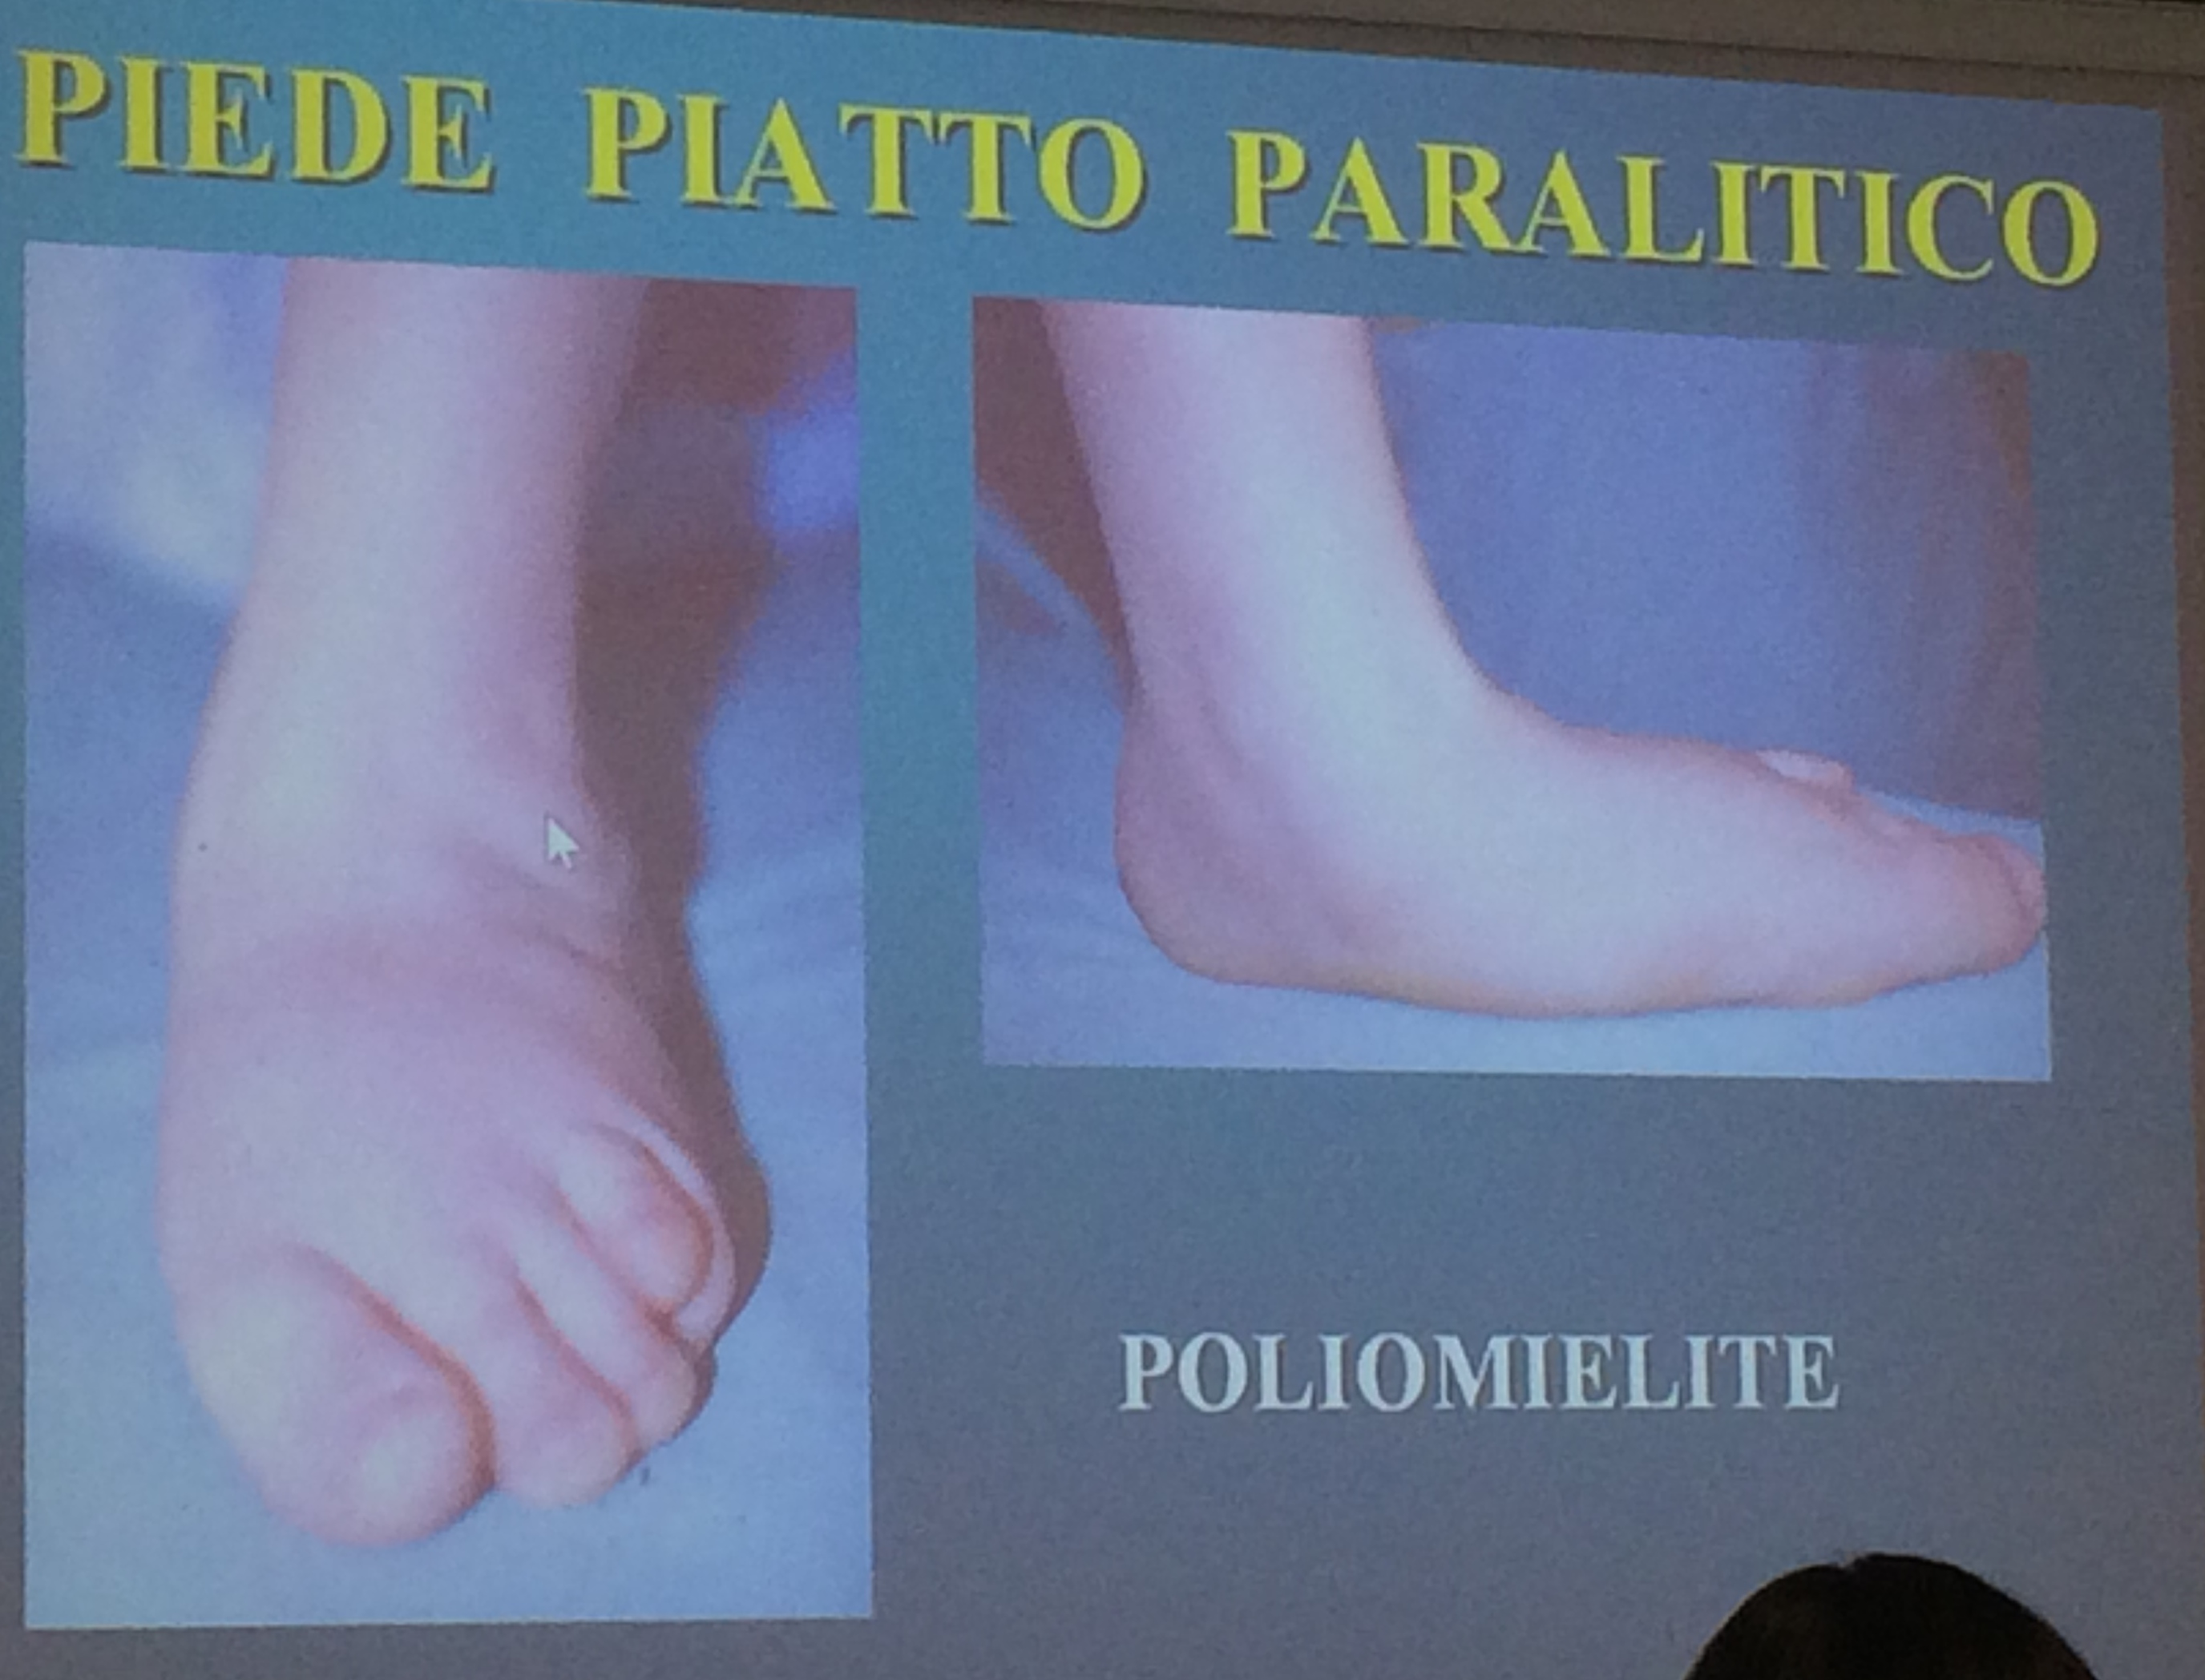
\includegraphics[width=0.4\textwidth]{014/image12.jpeg}
\end{figure}

\emph{Ricordiamo che il piede è in equilibrio quando i muscoli che si inseriscono su di esso hanno tutti lo stesso tono e la stessa trazione.} In questo forma
di piede piatto abbiamo un \emph{sovvertimento dell'equilibrio} fra i muscoli ad azione sul piede (si ripresenta poi nel piede cavo) \emph{da cui il sovvertimento dell'intera struttura}. Possiamo avere:

\begin{itemize}
\item
  \emph{Piede piatto paralitico}. Se abbiamo la paralisi di un muscolo possiamo avere un eccesso di pronazione con paralisi flaccide oppure paralisi spastiche o miopatie. Un caso può essere quello del piede piatto paralitico in corso di poliomielite.
\item
  \emph{Piede piatto spastico}. In seguito a paralisi cerebrale nei bambini possiamo avere il piede piatto spastico con contrattura continua (ipertono) dei peronei.
\end{itemize}

\subsection{Piede piatto da lassità legamentosa}

Non sempre ci sono situazioni troppo gravi. E' conseguenza della Sindrome di Ehler-Danlos, di Marfan, di Down, di Morquio, ecc....

\subsection{Piede piatto esito di piede torto congenito equino-varo-supinato}

Classico piede torto iper-corretto che evolve in piede piatto dove il valgismo è a livello della caviglia (\emph{valgismo della tibio-tarsica}). Seguono ad esempio agli interventi di Codivilla e di Turco. {[}N.B. Si preferisce parlare di \emph{iper-correzione} anche se viene detta iatrogena perché come ricorda il Prof. ``iatrogeno'' equivale a denuncia{]}

\begin{figure}[!ht]
\centering
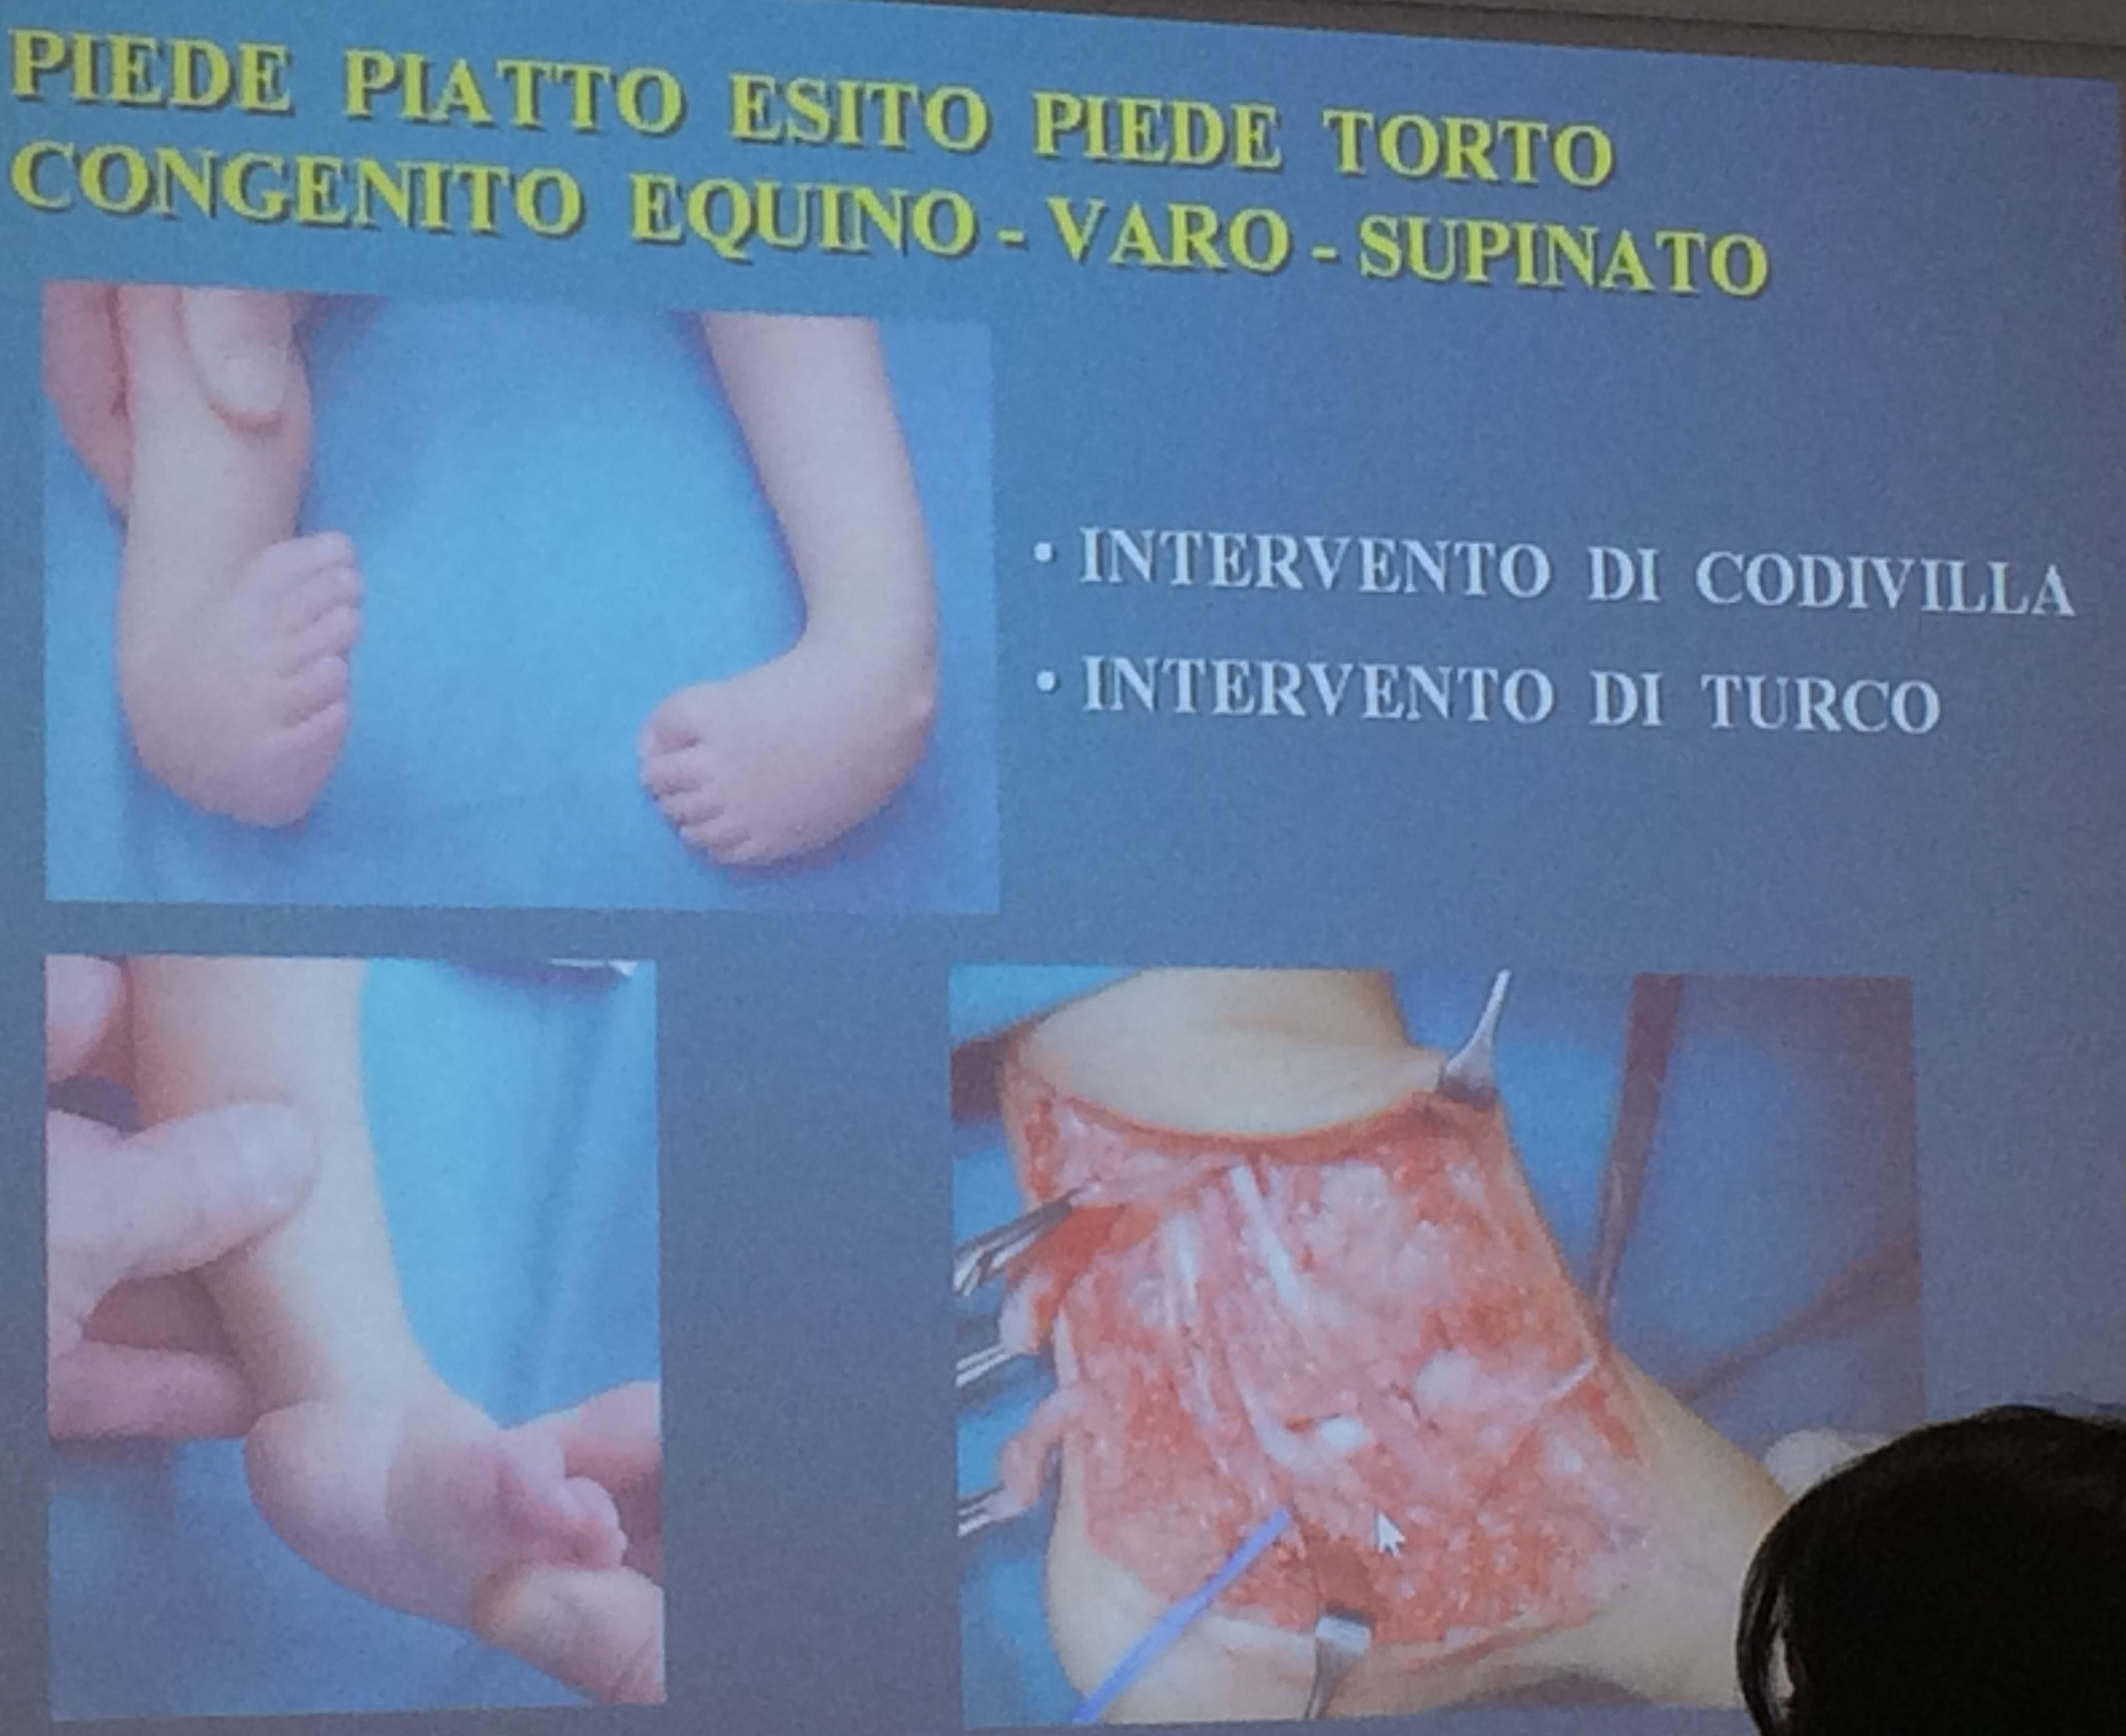
\includegraphics[width=0.4\textwidth]{014/image13.jpeg}
\end{figure}

\begin{figure}[!ht]
\centering
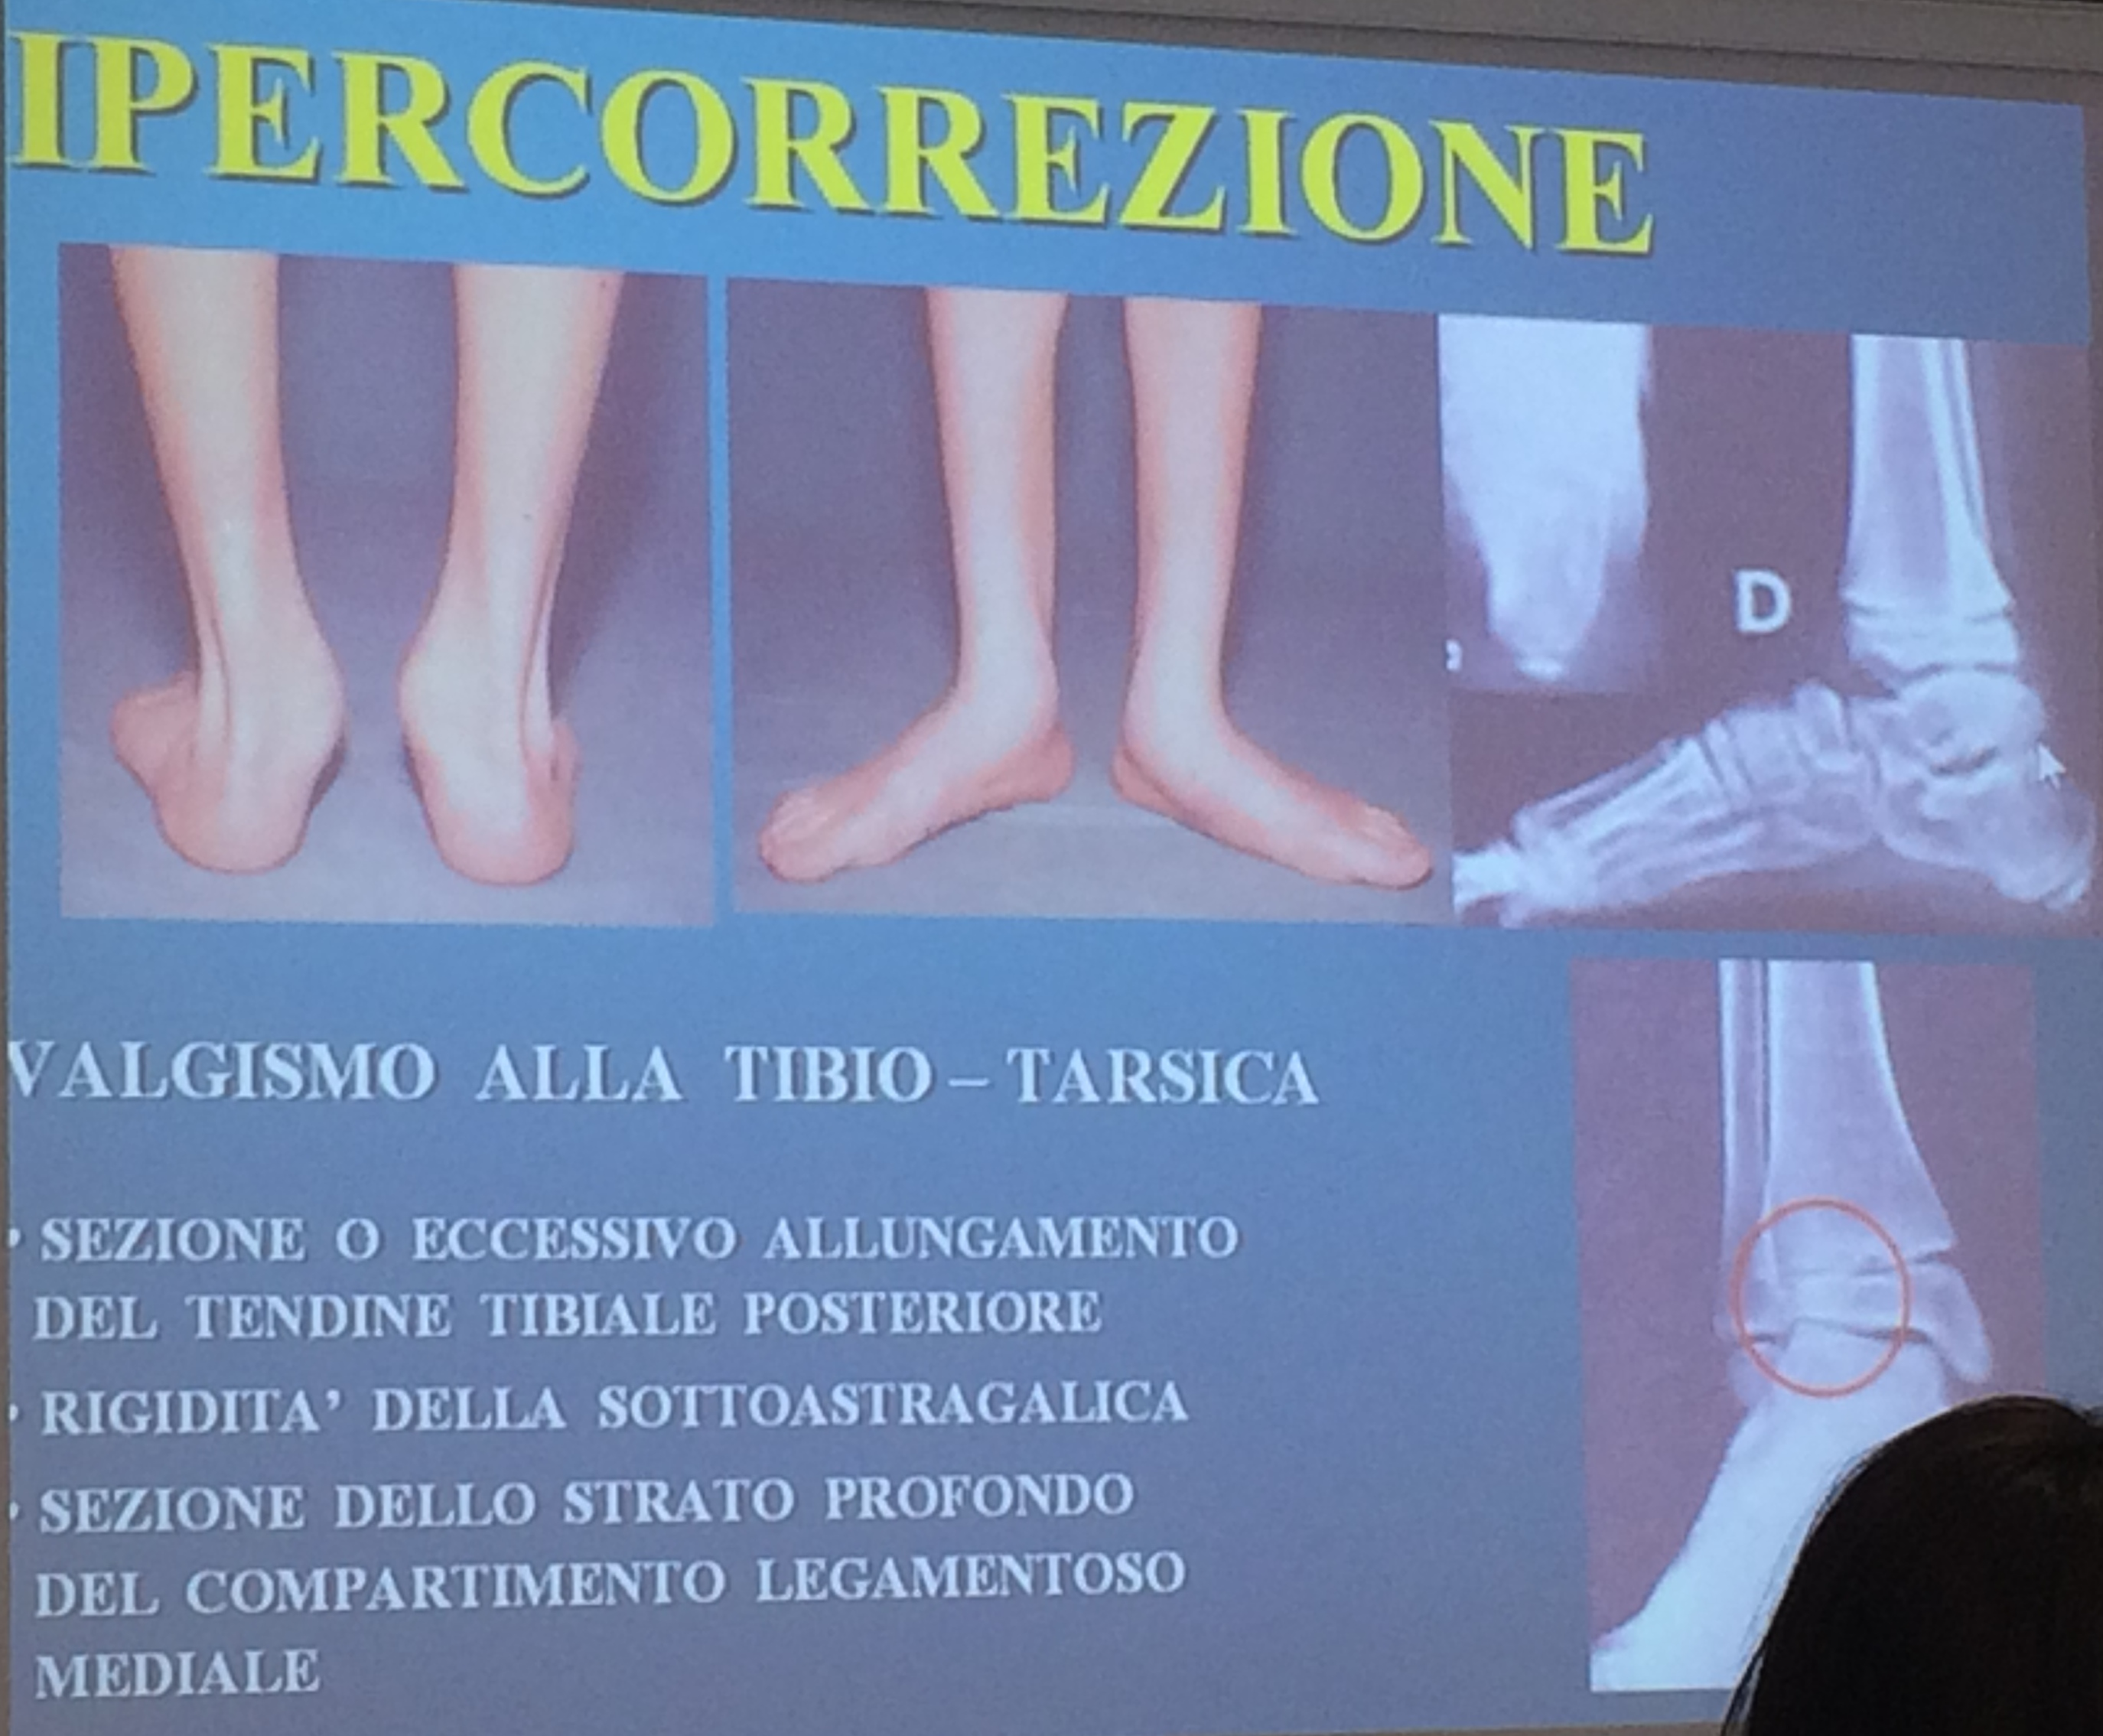
\includegraphics[width=0.4\textwidth]{014/image14.jpeg}
\end{figure}

DOMANDA: è possibile avere piede piatto in un solo piede? È raro, ma esiste. Anche quando lo sono entrambi, uno può essere modesto e l'altro più accentuato, ma dipende sempre dalla valutazione funzionale.
Solitamente anche se uno è grave, e l'altro è borderline, si operano entrambi i piedi.

N.B. L'argomento non è semplice come sembra, ma non chiederà nulla di estremamente specifico. Il Prof. ci tiene a far capire allo studente che non è tutto così facile come sembra, soprattutto per la questione del
trattamento che per molto tempo e ancora oggi viene relegato in modo semplicistico all'uso dei plantari.
